\tableofcontents

%


%\part{Alku}
\chapter{Esipuhe}

%%%%%%%%%%%%%%%%%%%%%%%%%%%%%%%%%%%%%%%%%%%%%%%%%%%%%%%%%%%%%%%%%%%%%%%%%%%%%%%%
%%%%  /usr/share/doc/texlive-fonts-extra-doc/fonts/arev/mathtesty.tex

% mathtesty.tex, by Stephen Hartke 20050522
% based on mathtestx.tex in the mathptmx package
% and symbols.tex by David Carlisle

Matematiikka tarjoaa työkaluja asioiden jäsentämiseen, päättelyyn ja mallintamiseen. Alasta riippuen käsittelemme matematiikassa erilaisia \textbf{objekteja}: Geometriassa tarkastelemme tasokuvioita ja kolmiulotteisia rakenteita. Algebra tutkii lukujen ja funktioiden ominaisuuksia. Todennäköisyyslaskenta arvioi erilaisten tapausten ja tilanteiden mahdollisuuksia ja riskejä. Matemaattinen analyysi (kurssit 7,8 ja 10) tutkii funktioita ja niiden muuttumista.

Jokaiseen tarkastelukohteeseen liitetään myös niille ominaisia \textbf{operaatioita}. Tämä kurssi käsittelee lähinnä lukuja ja niiden operaatioita, joita \textbf{laskutoimituksiksi} kutsutaan. Kirjan ensimmäisessä osassa käsittelemme luvun käsitteen, yleisimmät lukutyypit ja lukujen tavallisimman laskutoimitukset.

\section*{Sananen kirjasta}

Tulimme, kirjoitimme, voitimme.

\section*{Tekijöiden kommentit}

\todo{Miten olisi lyhyt kommentti tai lainaus jokaiselta tekijältä? Jotain yleviä mietteitä kirjasta, rohkaisevia tai nasevia kommentteja lukijalle, alku- tai loppukevennyksiä tai jotain randomia}

\textbf{Lauri Hellsten}\\

\\
\textbf{Niko Ilomäki}\\

\\
\textbf{Tero Keinänen}\\

\\
\textbf{Vesa Linja-aho}\\

\\
\textbf{Ossi Mauno}\\

\\
\textbf{Joonas Mäkinen}\\

\\
\textbf{Matti Pajunen}\\
Pitsa on paras :-D ja kokis
\\
\textbf{Pekka Peura}\\

\\
\textbf{Annika Piiroinen}\\

\\
\textbf{Kaisa Pohjonen\}\

\\
\textbf{Antti Rasila}\\

\\
\textbf{Johanna Rämö}\\

\\
\textbf{Juha Sointu}\\

\\
\textbf{Tommi Sottinen}\\

\\
\textbf{Jarno Talponen}\\

\\
\textbf{Topi Talvitie}\\

\\
\textbf{Sampo Tiensuu}\\

\\
\textbf{Ville Tilvis

\\

\section*{Kiitämme}
\begin{itemize}
\item Metropolia
\item Senja Larsen
\end{itemize}

%%%%%%%%%%%%%%%%%%%%%%%%%%%%%%%%%%%%%%%%%%%%%%%%%%%%%%%%%%%%%%%%%%%%%%%%%%%%%%%%
%%%% /usr/share/doc/texlive-doc-en/fonts/free-math-font-survey/source/textfragment.tex







%%% Local Variables: 
%%% mode: latex
%%% End: 


\part{Luvut ja laskutoimitukset}
\chapter{Numerot ja luvut}

(Joonas jatkaa tästä vielä!)

Matematiikka tarjoaa työkaluja asioiden jäsentämiseen, päättelyyn ja mallintamiseen. Alasta riippuen käsittelemme matematiikassa erilaisia \textbf{objekteja}: Geometriassa tarkastelemme tasokuvioita ja kolmiulotteisia rakenteita. Algebrassa tutkii lukujen ja funktioiden ominaisuuksia. Todennäköisyyslaskenta arvioi erilaisten tapausten ja tilanteiden mahdollisuuksia ja riskejä. Matemaattinen analyysi (kurssit 7,8 ja 10) tutkii funktioita ja niiden muuttumista.

Jokaiseen tarkastelukohteeseen liitetään myös niille ominaisia \textbf{operaatioita}. Tämä kurssi käsittelee lähinnä lukuja ja niiden operaatioita, joita \textbf{laskutoimituksiksi} kutsutaan. Aloitetaan yksinkertaisista määritelmistä: mitä tarkoittavat \textbf{numero} ja \textbf{luku}?

\laatikko{Länsimaisessa traditiossa käytössämme on kymmenen numeromerkkiä: 0, 1, 2, 3, 4, 5, 6, 7, 8 ja 9. Näitä kutsutaan hindu-arabialaisiksi numeroiksi.  }

Sanalla numero voidaan siis viitata yksittäiseen kirjoitettuun merkkiin. 

\laatikko{Luvut koostuvat numeroista.}
\begin{esimerkki}
Luku \[715531\] koostuu numeroista 7, 1, 5, 5, 3 ja 1.
\end{esimerkki}



Olennaista on myös...
lukujärjestelmä, paikkajärjestelmä

MIKSI KÄYTÄMME KIRJAIMIA?

suuruus, yhtäsuuruus, eri suuret

, ja Erilaisilla luvuilla voidaan suorittaa erilaisia laskutoimituksia. Seuraavissa luvuissa esitellään ja käydään läpi lukiomatematiikassa ja mahdollisissa jatko-opinnoissa käytettäviä lukujoukkoja ja tavallisimmat laskutoimitukset.


\chapter{Luonnolliset luvut}

(Joonas jatkaa tästä vielä!)

Suomen kielen verbi 'laskea' voi tarkoittaa matematiikassa kahta eri asiaa: lukumäärien laskemista ja laskutoimitusten suorittamista.

\laatikko{laskea (lukumäärä) englanti count ruotsi \_ /n
laskea (laskutoimitus) englanti calculate , ruotsi \_}

Ihmisellä ja muilla eläimillä on luonnostaan matemaattisia taitoja. Monet niistä, esimerkiksi lukumäärien laskeminen, ovat yllättävän monimutkaisia kognitiivisia prosesseja, jotka kehittyvät lapsuudessa – toisilla aiemmin, toisilla myöhemmin. Kaikki koulussa opeteltava peruslaskento ja myös matematiikka tieteen alana rakentavat tämän biologisen osaamisen päälle. Laskeminen itsessään on vain yksi matematiikan osa-alue, eikä kaikki matematiikka ole laskemista. Huomaa, että suomen kielen verbillä laskea tarkoitetaan sekä lukumäärien laskemista (engl. counting) että lukujen laskutoimitusten suorittamista (engl. calculating).

Hyvin olennaisena kehitysaskeleena niin yksilön matemaattiselle ajattelulle kuin yhteiskunnallekin on ollut luonnollisen kielen tavoin kyky merkitä lukumäärien laskemista ja muuta matemaattista pohdintaa kirjalliseen muotoon.  On olemassa hyvin monia erilaisia tapoja merkitä lukumääriä. Helpoin tapa ja yksinkertaisin tapa on käyttää vain yhtä samaa merkkiä ja toistaa sitä. Jos

käytettävissä olevien merkintöjä määrää voidaan lisätä, jolloin suuria lukuja voidaan kirjoittaa lyhyemmin. Tämä vastaa myös luonnollisten kielten tilannetta: Suomen kielen aakkosiin kuuluu 29 kirjainta, joista sanat muodostetaan. Sanat voivat olla kuinka pitkiä vain kahdesta kirjaimesta ylöspäin. Kiinassa sen sijaan käytetään omaa piirrosmerkkiä jokaiselle sanalle. Merkkejä täytyy osata 29 sijaan tuhansia, mutta jokaisen sanan voi kirjoittaa lyhyesti. 
Matematiikassa erilaisista numeromerkeistä tai yksinkertaisesti numeroista muodostetaan lukuja yhdistelemällä niitä sopivasti erilaisten paikkajärjestelmien mukaan. Esimerkiksi antiikin Roomassa käytössä olivat numeromerkit I, V, X, L, C , D ja M. Niiden numeroiden vastaavuudet meidän käyttämiimme lukuarvoihin ovat seuraavat:
I=1
V=5
X=10
L=50
C=100
D=500
M=1 000
Huomaa, että suuri osa roomalaisista numeromerkeistä ovat jo itsessään arvoltaan niin suuria, että me tarvitsemme niiden nykyilmaisuun monta merkkiä! Nollaa roomalaisissa numeroissa ei ole, ja tiettävästi tuhatta suurempia arvoja esittäviä numeromerkkejä merkkejä otettiin käyttöön vasta keskiajalla. 
Lukuja koostetaan näistä merkeistä siten, että merkit kirjoitetaan peräkkäin pääasiassa laskevassa järjestyksessä ja niiden numeroarvot lasketaan yhteen. Jos arvoltaan pienempi numeromerkki (korkeintaan yksi) edeltää suurempaa, pienempi vähennetään suuremmasta ennen yhteenlaskun jatkamista. 

% Luonnolliset luvut esitellään nyt kokonaislukujen alussa.

% \sivulaatikko{engl. \emph{natural numbers, counting numbers} ruots. \emph{naturliga tal}}
% 
% 
% \laatikko{Luonnollisia lukuja käytetään kolmeen eri tarkoitukseen:
% 
% \begin{enumerate}
% \item Lukumäärien ilmoittamiseen (kardinaaliluvut)
% \item Järjestyksen ilmoittamiseen (ordinaaliluvut)
% \item Indeksointiin ja asioiden nimeämiseen
% \end{enumerate}
% }


% \section{Tehtäviä}
% 
% \begin{tehtava}
% 
% Onko kardinaali vai ordinaali vai indeksointi?
% 
% \end{tehtava}

\chapter{Kokonaisluvut}

Yksinkertaisimmat käyttämämme luvut ovat lukumäärien ilmaisemiseen käytetyt $0,
1, 2, 3, \ldots$. Näitä kutsutaan \emph{luonnollisiksi luvuiksi}, ja niiden
joukkoa eli kaikkia luonnollisia lukuja yhdessä merkitään symbolilla
$\mathbb{N}$. Edellä nolla määriteltiin luonnolliseksi luvuksi, mutta tästä
ei ole yhteistä sopimusta: jotkut pitävät nollaa luonnollisena lukuna ja
toiset eivät.

Luonnollisille luvuille $m$ ja $n$ on määritelty yhteenlasku $m + n$, esimerkiksi
$5 + 3 = 8$.
Luonnollisten lukujen $m$ ja $n$ kertolasku määritellään peräkkäisinä yhteenlaskuina
\[m \cdot n = \underbrace{m + m + \ldots + m}_{n\text{ kpl}} = \underbrace{n + n + \ldots + n}_{m\text{ kpl}}.\]
Nollalla kertomisen ajatellaan olevan "tyhjä yhteenlasku"\ eli nolla,
$0 \cdot m = 0$.

Luonnollisten lukujen $m$ ja $n$ erotus määritellään yhteenlaskun avulla:
$m-n$ on luku $k$, jolle $k + n = m$. Kahden luonnollisen luvun erotus
ei kuitenkaan aina ole luonnollinen luku, esimerkkinä $3 - 5$.
Ratkaisemme ongelman määrittelemällä kullekin luonnolliselle
luvulle $n$ vastaluvun $-n$, jolle $n + (-n) = 0$.

Luonnolliset luvut ja niiden vastaluvut muodostavat yhdessä
kokonaislukujen joukon
\[\mathbb{Z} = \{\ldots, -2, -1, 0, 1, 2, \ldots\}.\]
Kun käytämme kokonaislukuja, voidaan kahden luvun erotus määritellä
yhteenlaskun ja vastaluvun avulla yksinkertaisesti $m-n = m+(-n)$.
\section{Kokonaislukujen laskusäännöt}

\section{Tiivistelmä}

    $a-(-b)=a+b$
    
    $-a\cdot (-b)=a\cdot b=ab$
    
    $-a:(-b)=a: b=a:b$

\section{Yhteen- ja vähennyslasku}

    Kysymys: Mitä saadaan, kun luvusta $5$ vähennetään luku $-8$?
    
    \laatikko{
        Määritelmä
        
        Jokaisella luvulla $a$ on vastaluku $-a$, jolle pätee $a+(-a)=0$.
    }
    
    Esimerkiksi luvun $2$ vastalukua merkitään $-2$, ja sille pätee $2+(-2)=0$.
    Vastaavasti luvun $-2$ vastaluku on sellainen luku, joka laskettuna yhteen
    luvun $-2$ kanssa antaa luvun $0$. Tämä on tietysti $2$, koska $-2+2=0$.
    Näin voidaan huomata, että $-(-2)=2$.
    
    Negatiivisten ja positiivisten lukujen yhteen- ja vähennyslaskut voidaan myös
    tulkita lukusuoran avulla.
    
    % tässä on vähän kyseenalaista käyttää sekaisin sanallista ja numeerista esitystä
    
    $5+8$ "viiteen lisätään $8$"
    
    \missingfigure{$5+8$ lukusuoralla}
    
    $5+(+8)$ "viiteen lisätään $+8$"
    
    $+8$ tarkoittaa samaa kuin $8$. '$+$'-merkkiä käytetään luvun edessä silloin,
    kun halutaan korostaa, että kyseessä on nimenomaan positiivinen luku.
    
    \missingfigure{$5+(+8)$ lukusuoralla}
    
    $5-(+8)$ "viidestä vähennetään $+8$"
    
    Tämä tarkoittaa samaa kuin 5-8. Lukusuoralla siis liikutaan 8 pykälää taaksepäin.
    
    \missingfigure{$5-(+8)$ lukusuoralla}
    
    $5+(-8)$ "viiteen lisätään $-8$"
    
    Mitä tapahtuu, kun lisätään negatiivinen luku? Kun lukuun lisätään 1, se
    kasvaa yhdellä. Kun lukuun lisätään 0, se ei kasva lainkaan. Eikö tällöin
    ole luonnollista ajatella, että kun lisätään luku, joka on pienempi kuin
    nolla, täytyisi lopputuloksesta tulla vielää pienempi. Tällä logiikalla
    negatiivisen luvun lisäämisen pitäisi siis pienentää alkuperäistä lukua.
    Siksi on sovittu, että $5+(-8)$ on yhtä suuri kuin $5-8$.
    
    \missingfigure{$5+(-8)$ lukusuoralla}
    
    $5-(-8)$ "viidestä vähennetään $-8$"
    
    Negatiivisen luvun lisääminen on vastakohtainen positiivisen luvun lisäämiselle.
    Tällöin olisi luonnollista, että negatiivisen luvun vähentäminen olisi myös
    vastakohtaista positiivisen luvun vähentämiselle. Kun positiivisen luvun
    vähentäminen pienentää lukua, pitäisi negatiivisen luvun vähentämisen siis
    kasvattaa lukua. Tämän vuoksi onkin sovittu, että $5-(-8)$ tarkoittaa samaa
    kuin $5+8$.
    
    \missingfigure{$5-(-8)$ lukusuoralla}
    
    Samaan logiikkaan perustuen on sovittu myös merkkisäännöt positiivisten ja
    negatiivisten lukujen kertolaskuissa. Kun negatiivinen ja positiivinen luku
    kerrotaan keskenään, saadaan negatiivinen luku, mutta kun kaksi negatiivista
    lukua kerrotaan keskenään, saadaan positiivinen luku.

\section{Kertolasku}

    $3 \cdot 4$ "kolme kappaletta nelosia"
    
    \missingfigure{$3 \cdot 4$ lukusuoralla}
    
    $3 \cdot (-4)$ "kolme kappaletta miinus-nelosia"
    
    \missingfigure{$3 \cdot (-4)$ lukusuoralla}
    
    $-3 \cdot 4$ "miinus-kolme kappaletta nelosia"
    
    \missingfigure{$-3 \cdot 4$ lukusuoralla}
    
    $-3 \cdot (-4)$ "miinus-kolme kappaletta miinus-nelosia"
    
    \missingfigure{$-3 \cdot (-4)$ lukusuoralla}

\section{Jakolasku}

Jakolaskua sanotaan kertolaskun käänteistoimitukseksi, koska se tekee tekee saman toimituksen kuin kertolasku, mutta vastakkaiseen suuntaan. Esimerkiksi $100:5\cdot 5=100$ ja $792\cdot 132:132=792$. Kun ensin kerrotaan jollain luvulla, ja sitten jaetaan samalla luvulla, päädytään takaisin samaan, mistä lähdettiin. Luonnollisesti olisi mukavaa, jos tämä ominaisuus säilyisi myös silloin, kun jaetaan ja kerrotaan negatiivisia lukuja. Tämän vuoksi jakolaskulle on sovittu samat merkkisäännöt kuin kertolaskulle, eli kaksi miinusmerkkiä kumoavat toisensa.

Esimerkiksi haluamme, että $(-12):(-3)\cdot (-3)=-12$. Nyt voimme kysyä, mitä laskun $(-12):(-3)$ tulokseksi pitäisi tulla, jotta jakolasku ja kertolasku säilyvät toisilleen käänteisinä, eli mikä luku kerrottuna $-3$:lla on $-12$. Kertolaskun merkkisäännöistä nähdään helposti, että tämän luvun täytyy olla $+4$ eli $4$. Niinpä on sovittu, että $(-12):(-3)=12:3=4$.

\begin{tehtava}
Kirjoita laskutoimitukseksi. (Laskuun ei tarvitse merkitä yksikköjä, eli celciusasteita tai euroja.)
\begin{enumerate}[a)]
\item Pakkasta on aluksi $-10^{\circ}$C ja sitten se lisääntyy kaksi (pakkas)astetta.
\item Pakkasta on aluksi $-20^{\circ}$C ja sitten se hellittää (vähentyy) kolme (pakkas)astetta.
\item Lämpötila on aluksi $17^{\circ}$C ja sitten se vähentyy viisi astetta.
\item Lämpötila on aluksi $5^{\circ}$C ja sitten se kasvaa kuusi astetta.
\item Mies on velkaa $30 000$ \euro mafialle ja kuolee. Hänen kolme poikaansa jakavat velan tasan keskenään. Kuinka paljon kukin on velkaa mafialle? Merkitse velkaa negatiivisella luvulla.
\end{enumerate}
\begin{vastaus}
\begin{enumerate}[a)]
\item $-10+(-2)=-12$
\item $-20-(-3)=-17$
\item $17-5=12$
\item $5+6=11$
\item $\frac{-30 000}{3}=10 000$
\end{enumerate}
\end{vastaus}
\end{tehtava}


\begin{tehtava}
Laske
\begin{enumerate}[a)]
    \item $1+1$
    \item $11+(-14)$
    \item $-8-(-4)$
    \item $-9-(+7)$
    \item $-(-8)+(5)-(-(-11))$
    \item $-8:(-4)$
    \item $(-8):(-4)$
    \item $(-5)\cdot 12$
\end{enumerate}
    \begin{vastaus}
    \begin{enumerate}[a)]
        \item $2$
        \item $-3$
        \item $-4$
        \item $-16$
        \item $2$
        \item $2$
        \item $2$
        \item $-60$
    \end{enumerate}
    \end{vastaus}
\end{tehtava}

\begin{tehtava}
Laske
\begin{enumerate}[a)]
\item $3+5$
\item $10-5-6+1$
\item $2 \cdot 2 - 1$
\item $-9 - 5 \cdot (-2) + 3$
\item $10 \cdot (5 - 2)$
\item $(2-5)(5 - 1) + 1$
\item $-9 - 2 \cdot ( 3 - 2 \cdot (3\cdot2 - 1))$
\end{enumerate}
\begin{vastaus}
\begin{enumerate}[a)]
\item $3$
\item $0$
\item $3$
\item $4$
\item $30$
\item $-11$
\item $5$
\end{enumerate}
\end{vastaus}
\end{tehtava}
\chapter{Jaollisuus \& tekijät}

\laatikko{
Määritelmä

Kokonaisluvun $a$ sanotaan olevan jaollinen kokonaisluvulla $b$, jos on olemassa sellainen kokonaisluku $c$, että $a=b\cdot c$. Tällöin sanotaan myös, että $b$ on $a$:n tekijä ja $c$ on $a$:n tekijä.
}

Esimerkiksi luku $-12$ on jaollinen luvulla $3$, koska $-12=3\cdot (-4)$. Toisaalta luku $-12$ ei ole jaollinen luvulla $5$, koska ei ole mitään kokonaislukua, joka kerrottuna viidellä olisi $12$.

Jaollisuuden voi ajatella myös jakolaskun avulla niin, että esim. luku $12$ on jaollinen luvulla $3$, koska luku $12$ voidaan jakaa $3$ yhtäsuureen osaan niin, että jokaisen osan koko on kokonaisluku -- tässä tapauksessa $4$.

Selvästi voidaan huomata, että kaikki luvut ovat jaollisia itsellään ja luvulla $1$. Esimerkiksi $37=37*1=1*37$, joten $37$ on jaollinen $1$:llä ja $37$:llä. Muita tekijöitä luvulla ei välttämättä ole.

\laatikko{
Määritelmä

Ykköstä suurempaa kokonaislukua sanotaan alkuluvuksi, jos sillä ei ole muita tekijöitä kuin $1$ ja luku itse.
}

Kokeilemalla havaitaan helposti, että esimerkiksi luvut 2, 3, 5, 7, 11, 13, 17 ja 19 ovat alkulukuja. 

\laatikko{
Aritmetiikan peruslause

Jokainen ykköstä suurempi kokonaisluku voidaan esittää yksikäsitteisesti alkulukujen tulona.
}

Esimerkiksi luku $84$ voidaan kirjoittaa muodossa $2\cdot 2\cdot 3\cdot 7$. Kokeilemalla huomataan helposti, että 2, 3, ja 7 ovat kaikki alkulukuja. Aritmetiikan peruslauseen nojalla tiedetään, että tämä on ainoa tapa kirjoittaa $84$ alkulukujen tulona - mahdollista kertolaskujärjestyksen vaihtoa lukuunottamatta. Kun luku $84$ esitetään muodossa $2\cdot 2\cdot 3\cdot 7$ on tapana sanoa, että se on jaettu alkutekijöihin. Alkutekjät esitetään yleensä kasvavassa numerojärjestyksessä. Jos sama luku esiintyy tekijöissä useampaan kertaan, on se yleensä yleensä tapana merkitä potenssina. Tällöin luku $84$ voitaisiin kirjoittaa tekijöihin jaettuna $2^2\cdot 3\cdot 7$ ja luku $96$ muodossa $2\cdot 2\cdot 2\cdot 2\cdot 2\cdot 3=2^5\cdot 3$
\chapter{Rationaaliluvut ja laskusäännöt}

\laatikko{
Rationaaliluvulla tarkoitetaan sellaista lukua, jonka voi esittää kahden kokonaisluvun osamääränä eli jakolaskuna.
}

Esimerkiksi luku $5$ on rationaaliluku, koska se saadaan laskutoimituksesta $5:1$ tai $15:3$ tai $(-20):(-4)$ tai monesta muustakin laskutoimituksesta.

Samoin luku $-7$ on rationaaliluku, koska se saadaan esimerkiksi laskutoimituksesta $(-14):2$.

\laatikko{
Jos nimittäjässä on eri luku, murtoluvut pitää ensin kertoa samannimisiksi eli \emph{laventaa}, jotta ne voi laskea yhteen.
\begin{equation}
\frac{a}{b} + \frac{c}{d} = \frac{ad}{bd} + \frac{bc}{bd} = \frac{ad+bc}{bd}
\end{equation}
}

Kumpi lapsi saa enemmän pizzaa: tyttö, joka saa kaksi kolmasosasiivua ($ \frac{2}{3}$) vai poika, joka saa kolme neljäsosasiivua ($ \frac{3}{4}$)? Huomataan että $4*3=12$. Jos ajatellaankin kummankin siivuja kahdestatoistaosina, osuuksia on helpompi vertailla. Tyttö saa kahdeksan kahdestoistaosaa, koska $ \frac{2}{3} = \frac{2 \cdot 4}{3 \cdot 4} = \frac{8}{12}$. Poika saa yhdeksän kahdestatoistaosaa, koska $ \frac{3}{4} = \frac{3 \cdot 3}{3 \cdot 4} = \frac{9}{12}$. Poika saa siis enemmän.

\missingfigure{tähän kuva pizzoista}

\laatikko{
Kokonaisluvun voi esittää murtolukuna asettamalle sen nimittäjäksi luvun yksi.
\begin{equation}
2 + \frac{1}{3} = \frac{2}{1} + \frac{1}{3} = \frac{3 \cdot 2}{3 \cdot 1} + \frac{1}{3} = \frac{6+1}{3} = \frac{7}{3}
\end{equation}
}

Kaksi ja yksi kolmasosa karkkipussillista karkkia on sama määrä pahoinvointia kuin seitsemän kolmasosakarkkipussillista karkkia.

\todo{enemmän asiaa prosenteista}

Yksi prosentti vastaa yhtä sadasosaa: $1 \% = \frac{1}{100}$

Laske %aika randomit luvut
\begin{tehtava}
    a) $\frac{6}{2} + \frac{3}{5}$
    b) $\frac{7}{8} - \frac{1}{4}$
    c) $2 \frac{1}{3} + \frac{4}{6}$
    d) $4 \frac{7}{2} - 6 \frac{5}{4}$
    
    \begin{vastaus}
        a) $\frac{18}{5}$
        b) $\frac{5}{8}$
        c) $3$
        d) $-\frac{41}{6}$
    \end{vastaus}
\end{tehtava}

\begin{tehtava}
    a) $\frac{1}{3} \cdot \frac{6}{5}$
    b) $\frac{5}{4} \cdot (-\frac{2}{3})$
    c) $\frac{2}{5} (2 - \frac{3}{4})$
    c) $(\frac{5}{6} - \frac{1}{3})(\frac{7}{4} - \frac{3}{2})$
    
    \begin{vastaus}
        a) $\frac{2}{5}$
        b) $\frac{5}{6}$
        c) $\frac{1}{2}$
        d) $\frac{1}{8}$
    \end{vastaus}
\end{tehtava}

\begin{tehtava} %lisää kakkaa
    a) $ \frac{\frac{3}{7} + \frac{5}{4}}{3}$
    b) $ \frac{\frac{10}{8}}{\frac{5}{2}}$
    c) $ \frac{\frac{1}{3} - \frac{5}{10}}{\frac{3}{4} + \frac{1}{2}}$
    d) $ 3\frac{\frac{4}{2} + \frac{10}{4}}{\frac{3}{2} - \frac{2}{3}}$
    
    \begin{vastaus}
        a) $\frac{47}{28}$
        b) $\frac{1}{2}$
        c) $-\frac{1}{3}$
        d) $\frac{54}{5}$
    \end{vastaus}
\end{tehtava}

\begin{tehtava} %lisää kakkaa
    Pontus, Viljami, Jarkko-Kaaleppi, Ahmed ja Milla leipoivat lanttuvompattipiirakkaa.
    Pontus kuitenkin söi piirakasta kolmanneksen ennen muita, ja loput piirakasta
    jaetaan muiden kanssa tasan. Kuinka suuren osan muut saavat?
    
    \begin{vastaus}
        Muut saavat piirakasta kuudesosan.
    \end{vastaus}
\end{tehtava}

\begin{tehtava} %ja lisää
    Huvipuiston sisäänpääsylippu maksaa 20 euroa, ja lapset pääsevät puoleen
    hintaan. Avajaispäivänä sisään pääsee 25\% halvemmalla. Kuinka paljon kolmen
    lapsen yksinhuoltajaperheelle maksaa päästä sisään avajaispäivänä?
    
    \begin{vastaus}
        37,50 euroa
    \end{vastaus}
\end{tehtava}

\chapter{Laskusäännöt ja lausekkeiden sieventäminen}



$a\cdot b:b=a$

$a:b\cdot b=a$

$a:b\cdot b=a$

\chapter{Laskusäännöt ja lausekkeiden sieventäminen}

\section{laskujärjestys}

\laatikko{
    \begin{enumerate}
        \item Sulut
        \item Potenssilaskut
        \item Kerto- ja jakolaskut vasemmalta oikealle
        \item Yhteen- ja jakolaskut vasemmalta oikealle
    \end{enumerate}
}

\section{lausekkeiden sieventäminen}

Matemaattisia ongelmia ratkaistaessa kannattaa usein etsiä vaihtoehtoisia tapoja jonkin laskutoimituksen, lausekkeen tai luvun ilmaisemiseksi. Tällöin usein korvataan esimerkiksi jokin laskutoimitus toisella laskutoimituksella, josta tulee sama tulos. Näin lauseke saadaan sellaiseen muotoon, jonka avulla ratkaisussa päästään eteenpäin.

Matematiikassa on tapana ajatella niin, että saman luvun voi kirjoittaa monella eri tavalla. Esimerkiksi merkinnät $42$, $-(-42)$, $6\cdot 7$ ja $(50-29)\cdot 2$ tarkoittavat kaikki samaa lukua. Niinpä missä tahansa lausekkeessa voi luvun $42$ paikale kirjoittaa merkinnän $(50-29)\cdot 2$, sillä ne tarkoittavat samaa lukua. Tähän lukuun on koottu sääntöjä, joiden avulla laskutoimituksia voi vaihtaa niin, että lopputulos ei muutu.

\laatikko{
Yhteenlaskut voi laskea missä järjestyksessä tahansa

$a+b=b+a$ (vaihdantalaki)

$a+(b+c)=(a+b)+c=a+b+c$ (liitäntälaki)
}

Esimerkiksi laskemalla voidaan tarkistaa, että $5+7=7+5$ ja että $(2+3)+5=2+(3+5)$.

Nämä säännöt voi yhdistää yleiseksi säännöksi, jonka mukaan laskujärjestystä voi vaihtaa ihan miten vain niin kauan kuin lausekkeessa on pelkkää yhteenlaskua.

Tämän säännön voi yleistää koskemaan myös vähennyslaskua, kun muistetaan, että vähennyslasku tarkoittaa oikeastaan käänteisluvun lisäämistä. $5-8$ tarkoittaa siis samaa kuin $5+(-8)$, joka voidaan nyt kirjoittaa yhteenlaskun vaihdantalain perusteella muotoon $(-8)+5$ eli $-8+5$ ilman, että laskun lopputulos muuttuu. Tästä seuraa seuraava sääntö:

\laatikko{
Pelkästään yhteen- ja vähennyslaskua sisältävässä lausekkeessa laskujärjestystä voi vaihtaa vapaasi, kun ajattelee miinusmerkin liikkuvan kuuluvan sitä seuraavaan lukuun ja liikkuvan sen mukana.
}

Esim. $5-8+7-2=5+(-8)+7+(-2)=(-2)+(-8)+5+7=-2-8+5+7$

Vastaavat säännöt pätevät kerto- ja jakolaskulle samoista syistä.

\laatikko{
Kertolaskut voi laskea missä järjestyksessä tahansa

$a\cdot b=b\cdot a$ (vaihdantalaki)

$a\cdot (b\cdot c)=(a\cdot b)\cdot c=a\cdot b\cdot c$ (liitäntälaki)
}

Jakolaskun voi ajatella käänteisluvulla kertomisena, eli

\laatikko{
Pelkästään kerto- ja jakolaskua sisältävässä lausekkeessa laskujärjestystä voi vaihtaa vapaasti, kun ajattelee jakolaskun käänteisluvulla kertomisena.
}

Esim. $5:8\cdot 7:2=5\cdot\frac18\cdot 7\cdot\frac12=7\cdot \frac12\cdot\frac18\cdot 5=7:2:8\cdot 5$

$a\cdot b:b=a$

$a:b\cdot b=a$

$a:b\cdot b=a$

\chapter{Desimaaliluvut}

\emph{Desimaaliluvut} on \emph{kymmenjärjestelmään} perustava tapa merkitä rationaalilukuja. Niillä voi merkitä myös irrationaalilukujen \emph{likiarvoja}.

\laatikko{
$123,456$ on esimerkki desimaaliluvusta.

\begin{itemize}
	\item $123$ on sen \emph{kokonaisosa}.
	\item Kokonaisluku erotetaan loppuosasta \emph{desimaalierottimella}, joka on Suomessa pilkku (,).
	\item Osaa $,456$ kutsutaan desimaaliluvun \emph{loppuosaksi}.
\end{itemize}

Esimerkkinä annettu desimaaliluku tulkitaan seuraavasti:
\begin{equation}
123,456 = 1 \cdot 10^2 + 2 \cdot 10^1 + 3 \cdot 10^0 + 4 \cdot 10^{-1} + 5 \cdot 10^{-2} + 6 \cdot 10^{-3}
\end{equation}

\missingfigure{Tähän kuva siitä, kuinka desimaaliluvun numerot vastaavat kymmenen potensseja}

Kymmenjärjestelmä saa nimensä siitä, että jokainen luvussa esiintyvä numero kertoo sen paikkaa vastaavien kymmenen potenssien määrän.
}

Desimaaliluvut voidaan muuttaa murtoluvuiksi laskemalla ne auki ylläolevan tavan mukaan.

\begin{esimerkki}
$21,37 = 2 \cdot 10^1 + 1 \cdot 10^0 + 3 \cdot 10^{-1} + 7 \cdot 10^{-2} = 2 \cdot 10 + 1 \cdot 1 + 3 \cdot \frac{1}{10} + 7 \cdot \frac{1}{100} = 21 + \frac{3}{10} + \frac{7}{100} = \frac{21 \cdot 100}{100} + \frac{3 \cdot 10}{10 \cdot 10} + \frac{7}{100} = \frac{21 \cdot 100 + 3 \cdot 10 + 7}{100} = \frac{2100+30+7}{100} = \frac{2137}{100}$
\end{esimerkki}

Toisaalta päästään paljon helpommalla, kun huomataan, että voidaan vain kertoa ja jakaa koko luku "niin monella kympillä, kuin on numeroita desimaalipilkun jälkeen". Täsmällisemmin sanottuna $10^n$:llä, jossa $n$ on pilkun jälkeen tulevien numeroiden määrä.

\begin{esimerkki}
$21,47 = 21,47 \cdot 1 = 21,47 \cdot \frac{10^2}{10^2} = \frac{21,47 \cdot 100}{100} = \frac{2147}{100}$
\end{esimerkki}

\begin{esimerkki}
$0,007 = 0,007 \cdot 1 = 0,007 \cdot \frac{10^3}{10^3} = \frac{0,007 \cdot 1000}{1000} = \frac{7}{1000}$
\end{esimerkki}

Menetelmän toimivuus kaikkien desimaalilukujen tapauksessa voidaan todistaa tarkastelemalla desimaaliluvun määritelmää, mutta jätetään tässä tekemättä.

\laatikko{
Tässä on joitain murtolukujen desimaaliesityksiä, jotka on hyvä osata
\begin{itemize}
	\item $ \frac{1}{10} = 0,1$
	\item $ \frac{1}{100} = 0,01$
	\item $ \frac{1}{2} = 0,5$
	\item $ \frac{1}{4} = 0,25$
	\item $ \frac{3}{4} = 0,75$
\end{itemize}
}

\begin{tehtava}
Laske ja totea edellä olevien murtolukujen desimaaliesitysten paikkansapitävyys.
\end{tehtava}

\begin{tehtava}
Muuta rationaaliluvuksi.
	\begin{enumerate}[a)]
		\item $43,532$
		\item $5,031$
		\item $0,23$
		\item $0,3002$
		\item $0,101$
	\end{enumerate}
\begin{vastaus}
	\begin{enumerate}[a)]
		\item $ \frac{43532}{1000}$
		\item $ \frac{5031}{1000}$
		\item $ \frac{23}{100}$
		\item $ \frac{3002}{1000}$
		\item $ \frac{101}{1000}$
	\end{enumerate}
\end{vastaus}
\end{tehtava}

\begin{tehtava}
Muuta rationaaliluvuksi.
	\begin{enumerate}[a)]
		\item $0,01$
		\item $0,0245$
		\item $0,003$
		\item $0,001004$
	\end{enumerate}
\begin{vastaus}
	\begin{enumerate}[a)]
		\item $ \frac{1}{100}$
		\item $ \frac{245}{1000}$
		\item $ \frac{3}{1000}$
		\item $ \frac{1004}{1 000 000}$
	\end{enumerate}
\end{vastaus}
\end{tehtava}

\todo{rat.lukujen muuttaminen desimaaliluvuiksi, motivaatio, teoria ja esimerkkejä}
\todo{tehtäviä rat.lukujen muuttamisesta desimaaliluvuiksi (huom! ei päättymättömiä desimaaliluvuista)}

\begin{tehtava}
	\begin{enumerate}[a)]
		\item
	\end{enumerate}
\begin{vastaus}
	\begin{enumerate}[a)]
		\item
	\end{enumerate}
\end{vastaus}
\end{tehtava}

\begin{tehtava}
	\begin{enumerate}[a)]
		\item
	\end{enumerate}
\begin{vastaus}
	\begin{enumerate}[a)]
		\item
	\end{enumerate}
\end{vastaus}
\end{tehtava}

\laatikko{
Joissain yhteyksissä käytetään muitakin \emph{lukujärjestelmiä} kuin kymmenjärjestelmää. Esimerkiksi tietokoneet käyttävät kaksikantajärjestelmää eli \emph{binäärijärjestelmää}. Binäärijärjestelmässä jokainen luvun numero kertoo sen paikkaa vastaavan kakkosen potenssien määrän kymmenen potenssien sijasta.

Binäärijärjestelmässä esitetty luku merkitään yleensä kirjoittamalla pieni kakkonen luvun jälkeen, esim. $12,34_2$.
}

\begin{esimerkki}
$12,34_2 = 1 \cdot 2^1 + 2 \cdot 2^0 + 3 \cdot 2^{-1} + 4 \cdot 2^{-2}$
\end{esimerkki}

\todo{pari helppoa muuntotehtävää binääriluvuista kymmenjärjestelmään}
\todo{pari ekstrahellpoa muuntotehtävää kymmenjärjestelmästä binääriin (huom! ei päättymättömiä binäärilukuja)}

\begin{tehtava}
	\begin{enumerate}[a)]
		\item
	\end{enumerate}
\begin{vastaus}
	\begin{enumerate}[a)]
		\item
	\end{enumerate}
\end{vastaus}
\end{tehtava}

\begin{tehtava}
	\begin{enumerate}[a)]
		\item
	\end{enumerate}
\begin{vastaus}
	\begin{enumerate}[a)]
		\item
	\end{enumerate}
\end{vastaus}
\end{tehtava}

\todo{päättymättömät desimaaliluvut, jotka on esitettävissä rationaalilukuina}
\todo{nämä on hyvä osata: esimerkkejä desimaaliluvuista jotka on esitettävissä rationaalilukuina, esim. 0,333...}
\todo{tehtäviä päättymättömistä mutta jaksollisista desimaaliluvuista}
\chapter{Potenssisäännöt}

Jos $a$ on reaaliluku ja $n$ on luonnollinen luku, potenssilla $a^n$ tarkoitetaan tuloa
\[
a^n = \underbrace{a\cdot \ldots \cdot a}_{n\text{ kpl}}. 
\]
Lukua $a$ kutsutaan potenssin \emph{kantaluvuksi} ja lukua $n$ \emph{eksponentiksi}. Luvun toista potenssia $a^2$ kutsutaan myös luvun $a$ \emph{neliöksi} ja kolmatta potenssia $a^3$ sen \emph{kuutioksi}. Luvun $a>0$ neliö on sellaisen neliön pinta-ala, jonka sivun pituus on $a$. Vastaavasti, jos kuution särmän pituus on $a$, niin $a^3$ on kuution kyseisen tilavuus.

\begin{esimerkki}
Laske $2^4$.

{\bf Ratkaisu.}
Potenssissa $2^4$ luku $2$ on kantaluku ja luku $4$ on eksponentti.
Merkinnällä $2^4$ siis tarkoitetaan tuloa $2\cdot 2\cdot 2\cdot 2$. Siten
\[
2^4=2\cdot 2\cdot 2\cdot 2=16.
\]

{\bf Vastaus.} $16$.
\end{esimerkki}

Potensseille pätevät seuraavat laskusäännöt.

\laatikko{
{\bf Potenssien laskusääntöjä}

Olkoot $m$ ja $n$ kokonaislukuja ja $a$ reaaliluku.

\begin{tabular}{ll}
$a^m\cdot a^n = a^{m+n}$ & Samakantaisten potenssien tulo\\
$\frac{a^m}{a^n} = a^{m-n}$, $a\neq 0,\,m>n$ &Samakantaisten potenssien osamäärä\\
$(a\cdot b)^n = a^n+b^n$ & Tulon potenssi\\
$\Big(\frac{a}{b}\Big)^n = \frac{a^n}{b^n}$, $b\neq 0$ & Osamäärän potenssi\\ 
$(a^m)^n = a^{m\cdot n}$ & Potenssin potenssi\\

\end{tabular}
}


\begin{esimerkki}
%\textbf{Esimerkki 1}
\begin{equation}
\text{a)} (-2)^3=(-2)\cdot (-2)\cdot (-2)=-8.
\end{equation}

\begin{equation}
\text{b)} (-2)^4=(-2)\cdot (-2)\cdot (-2)\cdot (-2)=16.
\end{equation}

\begin{equation}
\text{c)} -2^4=-2\cdot 2\cdot 2\cdot 2=-16.
\end{equation}

Potenssilla $2^4$ tarkoitetaan tuloa $2\cdot 2\cdot 2\cdot 2$. Eli
\begin{equation*}
2^4=2\cdot 2\cdot 2\cdot 2=16.
\end{equation*}
Lausekkeessa $2^4$ luku 2 on \textbf{kantaluku} ja luku 4 on \textbf{eksponentti}.


\begin{esimerkki}
Potenssit luvuilla.

a) $(-2)^3=(-2)\cdot (-2)\cdot (-2)=-8$

b) $(-2)^4=(-2)\cdot (-2)\cdot (-2)\cdot (-2)=16$

c) $-2^4=-(2^4)=-(2\cdot 2\cdot 2\cdot 2)=-16$

d) $2^2\cdot 2^3=\underbrace{2\cdot 2}_{2 kpl}\cdot \underbrace{2\cdot 2\cdot 2}_{3 \text{kpl}}=2^5=32$

e) $\frac{2^4\cdot 2^2}{2^3}=\frac{\overbrace{2\cdot 2\cdot 2\cdot \cancel{2}}\cdot \overbrace{\cancel{2}\cdot \cancel{2}}}{\cancel{2}\cdot \cancel{2}\cdot \cancel{2}}=2^3=8$
\end{esimerkki}

\section*{Potenssien laskusääntöjä}

\laatikko{
Samankantaisten potenssien kertolasku\\
a) $a^3\cdot a^4=\underbrace{a\cdot a\cdot a}_{3 kpl}\cdot \underbrace{a\cdot a\cdot a\cdot a}_{4 kpl}=a^{\mathbf{3+4}}=a^7$

Samankantaisten potenssien jakolasku\\
b) $\frac{a^7}{a^4}=\frac{a\cdot a\cdot a\cdot \cancel{a}\cdot \cancel{a}\cdot \cancel{a}\cdot \cancel{a}}{\cancel{a}\cdot \cancel{a}\cdot \cancel{a}\cdot \cancel{a}}=a^{\mathbf{7-4}}=a^3$

Potenssin potenssi\\
c) $(a^2)^3=\underbrace{a^2\cdot a^2\cdot a^2}_{3 kpl}=\underbrace{a\cdot a\cdot a\cdot a\cdot a\cdot a}_{2\cdot 3=6 kpl}=a^{\mathbf{2\cdot 3}}=a^6$

Tulon potenssi\\
d) $(ab^5)^3=ab^5\cdot ab^5\cdot ab^5=a\cdot a\cdot a\cdot b^5\cdot b^5\cdot b^5=a^{\mathbf{1\cdot 3}}\cdot b^{\mathbf{5\cdot 3}}=a^3b^{15}$

Osamäärän potenssi\\
e) $\left(\frac{a^9}{b^7}\right)^3=\frac{a^9}{b^7}\cdot \frac{a^9}{b^7}\cdot \frac{a^9}{b^7}=\frac{a^9\cdot a^9\cdot a^9}{b^7\cdot b^7\cdot b^7}=\frac{a^{\mathbf{9\cdot 3}}}{b^{\mathbf{7\cdot 3}}}=\frac{a^{27}}{a^{21}}$
}
\section*{Negatiivinen luku ja nolla eksponenttina}

Sievennetään osamäärä $\frac{a^3}{a^5}$ kahdella eri tavalla. Supistamalla yhteiset tekijät lopputulos

\begin{equation*}
\frac{a^3}{a^5}=\frac{\cancel{a}\cdot \cancel{a}\cdot \cancel{a}}{a\cdot a\cdot \cancel{a}\cdot \cancel{a}\cdot \cancel{a}}=\frac{1}{a\cdot a}=\boldsymbol{\frac{1}{a^2}}
\end{equation*}

on erinäköinen, kuin käyttämällä potenssien laskusääntöjä

\begin{equation*}
\frac{a^3}{a^5}=a^{3-5}=\boldsymbol {a^{-2}}{.}
\end{equation*}

Koska lähtötilanne on molemmissa tapauksissa sama, voidaan määritellä, että

\begin{equation}

\text{d)} 2^2\cdot 2^3=\underbrace{2\cdot 2}_{2\textrm{ kpl}}\cdot \underbrace{2\cdot 2\cdot 2}_{3\textrm{ kpl}}=2^5=32.
\frac{1}{x^2}=x^{-2}
x^{-2}=\frac{1}{x^2}
\end{equation}

\laatikko{Yleisesti määritellään (kun $x\neq 0$)
\begin{equation}
\text{e)}\frac{2^4\cdot 2^2}{2^3}=\frac{\overbrace{2\cdot 2\cdot 2\cdot \cancel{2}}\cdot \overbrace{\cancel{2}\cdot \cancel{2}}}{\cancel{2}\cdot \cancel{2}\cdot \cancel{2}}.
x^{-n}=\frac{1}{x^n}
\end{equation}
\begin{equation*}
	a^{-2}=\frac{1}{a^2}{.}
\end{equation*}

\laatikko{\textbf {Negatiivinen eksponentti} (kun $a\neq 0$).
\begin{equation*}
	a^{-n}=\frac{1}{a^n}
\end{equation*}
}

Kun eksponenttina on nolla, on tuloksena aina luku 1.

\begin{esimerkki}
$\frac{a^3}{a^3}=\frac{\cancel{a}\cdot \cancel{a}\cdot \cancel{a}}{\cancel{a}\cdot \cancel{a}\cdot \cancel{a}}=1$
	ja vastaavasti
$\frac{a^3}{a^3}=a^{3-3}=a^0${.}
\end{esimerkki}


\laatikko{\textbf{Eksponenttina nolla} (kun $a\neq 0$)
\begin{equation*}
a^{0}=1
\end{equation*}
}



% Tehtävät ovat tarkoitettu todella heikoille
%Näitä lienee liikaa. Karsitaanko vai siirretäänkö muualle?
%Tarvitaan myös haastavia tehtäviä.
Sievennä.
\begin{tehtava}
%Sievennä \quad
a) $a\cdot a\cdot a$ \quad b) $a\cdot a\cdot a\cdot b\cdot b\cdot b\cdot b$ \quad
c) $a\cdot b\cdot a\cdot b\cdot a\cdot b\cdot a$
\begin{vastaus}
a) $a^3$ \qquad b) $a^3b^4$ \qquad c) $a^4b^3$
\end{vastaus}
\end{tehtava}
\begin{tehtava}
%Sievennä \quad
a) $a^2\cdot a^3$ \qquad b) $a^3a^2$ \qquad c) $a^2 a$ \qquad d) $a a^2 a$ \qquad
e) $a^2a^1a^3$
\begin{vastaus}
a) $a^5$ \qquad b) $a^5$ \qquad c) $a^3$ \qquad d) $a^4$ \qquad e) $a^6$
\end{vastaus}
\end{tehtava}
\begin{tehtava}
%Sievennä \quad
a) $a^0$ \qquad b) $a^0a^0$ \qquad c) $a a^1$ \qquad d) $aa^0$ \qquad
e) $a^0a^1$
\begin{vastaus}
a) $1$ \quad ($a\neq0$, koska $0^0$ ei ole määritelty) \qquad b) $1$ \qquad c) $a$ \qquad d) $a^2$ \qquad
e) $a$
\end{vastaus}
\end{tehtava}
\begin{tehtava}
%Sievennä \quad
a) $a^1 a a^2$ \qquad b) $aaaa$ \qquad c) $a^3ba^2$ \qquad d) $aba^0ba^1$
\begin{vastaus}
a) $ a^4$ \qquad b) $a^4$ \qquad c) $a^5b$ \qquad d) $a^2b^2$
\end{vastaus}
\end{tehtava}
% teht 5
\begin{tehtava}
%Sievennä \quad
a) $(-2)\cdot(-2)\cdot(-2)$ \qquad b) $(-1)\cdot(-1)\cdot(-1)\cdot(-1)$
\begin{vastaus}
a) $ -8$ \qquad b) $1$
\end{vastaus}
\end{tehtava}
\begin{tehtava}
%Sievennä \quad
a) $(-a)\cdot(-a)$ \qquad b) $(-a)\cdot(-a)\cdot(-b)$ \qquad c) $(-a^2)\cdot(-a^2)$
\begin{vastaus}
a) $a^2$ \qquad b) $-a^2b$ \qquad c) $a^4$
\end{vastaus}
\end{tehtava}
\begin{tehtava}
%Sievennä \quad
a) $-a\cdot(-a)$ \qquad b) $-a\cdot(-a)\cdot(-b)$ \qquad c) $-a^2\cdot(-a^2)$
\begin{vastaus}
a) $a^2$ \qquad b) $-a^2b$ \qquad c) $a^4$
\end{vastaus}
\end{tehtava}
\begin{tehtava}
%Sievennä \quad
a) $-a^3\cdot(-a^2)$ \qquad b) $a\cdot(-a)\cdot(-b)$ \qquad c) $a^2\cdot(-a^2)$
\begin{vastaus}
a) $a^5$ \qquad b) $a^2b$ \qquad c) $-a^4$
\end{vastaus}
\end{tehtava}
\begin{tehtava}
%Sievennä \quad
a) $2^3\cdot2^3$ \qquad b) $4^3$ \qquad c) $(2^2)^3$ \qquad d) $2^{2+2+2}$
\begin{vastaus}
a) $64$ \qquad b) $64$ \qquad c) $64$ \qquad d) $64$
\end{vastaus}
\end{tehtava}
%teht. 10
\begin{tehtava}
%Sievennä \quad
a) $0^3\cdot0^3\cdot0^3$ \qquad b) $3^1$ \qquad c) $2^{2+3}$ \qquad d) $2^{6-4}$ \qquad e) $5^0$
\begin{vastaus}
a) $1$ \qquad b) $3$ \qquad c) $32$ \qquad d) $4$ \qquad e) $1$
\end{vastaus}
\end{tehtava}
\begin{tehtava}
%Sievennä \quad
a) $(a^3)^1$ \qquad b) $(a^6)^2$ \qquad c) $(a^2)^4$ \qquad d) $(a^1)^3$ \qquad e) $(a^0)^5$
\begin{vastaus}
a) $a^3$ \qquad b) $a^{12}$ \qquad c) $a^8$ \qquad d) $a^3$ \qquad e) $1$
\end{vastaus}
\end{tehtava}
\begin{tehtava}
%Sievennä \quad
a) $a^3\cdot a^2\cdot a^5$ \qquad b) $(a^3)^2$ \qquad c) $(a^2a^3)^4$ \qquad d) $a^{7-2}$
\begin{vastaus}
a) $a^{10}$ \qquad b) $a^6$ \qquad c) $a^{20}$ \qquad d) $a^5$
\end{vastaus}
\end{tehtava}
\begin{tehtava}
%Sievennä \quad
a) $(1\cdot a)^3$ \qquad b) $(a\cdot 2)^2$ \qquad c) $(-2abc)^3$ \qquad d) $(3a)^4$
\begin{vastaus}
a) $a^3$ \qquad b) $4a^2$ \qquad c) $-8a^3b^3c^3$ \qquad d) $91a^4$
\end{vastaus}
\end{tehtava}
\begin{tehtava}
%Sievennä \quad
a) $a^3\cdot b^2\cdot a^5$ \qquad b) $(-ab^3)^2$ \qquad c) $(a^5a^4)^3$ \qquad d) $b(ab)^2$
\begin{vastaus}
a) $a^8b^2$ \qquad b) $a^2b^6$ \qquad c) $a^{15}b^{12}$ \qquad d) $a^2b^3$
\end{vastaus}
\end{tehtava}
%teht.15
\begin{tehtava}
%Sievennä \quad
a) $b^3(ab^0)^2$ \qquad b) $(ab^3)^0$ \qquad c) $(aa^4)^3a^2$ \qquad d) $a^3(b^2a)^5$
\begin{vastaus}
a) $a^2b^3$ \qquad b) $1$ \qquad c) $a^{17}$ \qquad d) $a^8b^{10}$
\end{vastaus}
\end{tehtava}
\begin{tehtava}
%Sievennä \quad
a) $(1^3\cdot 2^2)^2$ \qquad b) $(1^2\cdot 2^3)^2$ \qquad c) $(2^2a^4)^2$ \qquad d) $b(3b)^3$
\begin{vastaus}
a) $16$ \qquad b) $64$ \qquad c) $16a^8$ \qquad d) $27b^4$
\end{vastaus}
\end{tehtava}
\begin{tehtava}
%Sievennä \quad
a) $(a^3b^2)^2$ \qquad b) $a(a^2b^3)^4$ \qquad c) $(b^2a^4)^5$ \qquad d) $b(2ab^2)^3$
\begin{vastaus}
a) $a^6b^4$ \qquad b) $a^9b^{12}$ \qquad c) $a^{20}b^{10}$ \qquad d) $8a^3b^7$
\end{vastaus}
\end{tehtava}
\begin{tehtava}
%Sievennä \quad
a) $\frac{2^3}{2^2}$ \qquad b) $\frac{2^4}{2^2}$ \qquad c) $\frac{2^3}{2^1}$ \qquad d) $\frac{2^3}{2^0}$ \qquad e) $\frac{2^3}{2^4}$
\qquad f) $\frac{2^3}{2^5}$
\begin{vastaus}
a) $2$ \qquad b) $4$ \qquad c) $4$ \qquad d) $8$ \qquad e) $\frac{1}{2}$ \qquad f) $\frac{1}{4}$
\end{vastaus}
\end{tehtava}
\begin{tehtava}
%Sievennä \quad
a) $\frac{a^3}{a^2}$ \qquad b) $\frac{a^4}{a^2}$ \qquad c) $\frac{a^3}{a^1}$ \qquad d) $\frac{a^3}{a^0}$ \qquad e) $\frac{a^3}{a^4}$
\qquad f) $\frac{a^3}{a^5}$
\begin{vastaus}
a) $a$ \qquad b) $a^2$ \qquad c) $a^2$ \qquad d) $a^3$ \qquad e) $a^{-1} = \frac{1}{a}$ \qquad f) $a^{-2} = \frac{1}{a^2}$
\end{vastaus}
\end{tehtava}
%teht. 20
\begin{tehtava}
%Sievennä \quad
a) $\frac{a^2b^2}{ab}$ \qquad b) $\frac{a^2b}{a^2}$ \qquad c) $\frac{a^3}{a^3}$ \qquad d) $\frac{1}{a^0}$ \qquad e) $\frac{ab^3}{-b^4}$
\begin{vastaus}
a) $ab$ \qquad b) $b$ \qquad c) $1$ \qquad d) $1$ \qquad e) $-\frac{a}{b}$
\end{vastaus}
\end{tehtava}
Sievennä ja kirjoita potenssiksi, jonka eksponentti on positiivinen.
\begin{tehtava}
%Sievennä \quad
a) $a^{-3}$ \qquad b) $\frac{a}{a^3}$ \qquad c) $a^{-2}\cdot a^5$ \qquad d) $\frac{b}{a^4}b^{-4}$ \qquad e) $\frac{a^3}{a^{-5}}$
\begin{vastaus}
a) $\frac{1}{a^3}$ \qquad b) $\frac{1}{a^2}$ \qquad c) $a^3$ \qquad d) $\frac{}{a^4b^3}$ \qquad e) $a^8$
\end{vastaus}
\end{tehtava}
Esitä ilman sulkuja ja sievennä.
\begin{tehtava}
%Esitä ilman sulkuja ja sievennä \quad
a) $(\frac{1}{2})^2$ \qquad b) $(\frac{1}{3})^3$ \qquad c) $(\frac{a}{b})^4$ \qquad d) $(\frac{a^2}{b^3})^2$ \qquad
e) $\left(\frac{a^2}{ab^2}\right)^2$
\begin{vastaus}
a) $\frac{1}{4}$ \qquad b) $\frac{1}{27}$ \qquad c) $\frac{a^4}{b^4}$ \qquad d) $\frac{a^4}{b^6}$ \qquad e) $\frac{a^2}{b^4}$
\end{vastaus}
\end{tehtava}
\begin{tehtava}
%Esitä ilman sulkuja ja sievennä \quad
a) $(\frac{1}{2})\cdot(\frac{1}{2})$ \qquad b) $(-\frac{ab^2}{a^2b})^3$ \qquad c) $(-a^4b^4)^2$ \qquad d) $\left((\frac{a}{b})^4\right)^2$
\begin{vastaus}
a) $\frac{1}{4}$ \qquad b) $-\frac{b^3}{a^3}$ \qquad c) $a^8b^8$ \qquad d) $\frac{a^8}{b^8}$
\end{vastaus}
\end{tehtava}
\begin{tehtava}
%Esitä ilman sulkuja ja sievennä \quad
a) $\frac{6a^9}{3a^2}$ \qquad b) $(\frac{a^2b^{-2}}{a^2b})^{-3}$ \qquad c) $\frac{5a^2}{-15a}$ \qquad
d) $\left(-(\frac{10^3}{100b})^2 b^{-1} \right )^2$
\begin{vastaus}
a) $2a^7$ \qquad b) $b^9$ \qquad c) $-\frac{1}{3}a = -\frac{a}{3}$ \qquad d) $\frac{10\ 000}{b^6}$
\end{vastaus}
\end{tehtava}

\chapter{Murtolausekkeiden sieventäminen}

\begin{tehtava}
Sievennä
\begin{enumerate}
\item $\frac{2x^3}{x}$
\item $\frac{6x^2+8y}{2x^2}$
\item $ \frac{1-x}{3} + \frac{x+2}{6}$
\item $ \frac{5x-1}{3} - \frac{2x+5}{2}$
\end{enumerate}
\begin{vastaus}
\begin{enumerate}
\item $2x^2$
\item $3+4y$
\item $ -\frac{x}{6}$
\item $ \frac{2}{3} x - \frac{17}{6}$
\end{enumerate}
\end{vastaus}
\end{tehtava}


\chapter{Juuret}


\section{Neliöjuuri}

Ajatellaan, että neliön pinta-ala on $a$. Halutaan tietää, mikä on kyseisen neliön sivun pituus. Vastausta tähän kysymykseen kutsutaan luvun $a\ge 0$ neliöjuureksi ja merkitään $\sqrt{a}$. Luvun $a$ neliöjuuri on myös yhtälön $x^2 = a$ vastaus. Tällöin täytyy kuitenkin huomata, että myös luku $x=-\sqrt{a}$ toteutaa kyseisen yhtälön. Neliöjuurella tarkoitetaan kyseisen yhtälön epänegatiivista vastausta. Tämä on luonnollista, koska neliön sivun pituus ei voi olla negatiivinen luku.

\laatikko{Luvun $a$ neliöjuuri on epänegatiivinen luku, jonka neliö on $a$. Tämä voidaan ilmaista myös $(\sqrt{a})^2=a$.}

Neliöjuurta ei tällä kurssilla määritellä negatiivisille luvuille, koska neliön pinta-ala on aina positiivinen luku tai nolla. Käytännössä lukujen neliöjuuria lasketaan laskimella.


\begin{esimerkki}
Laske.
\begin{enumerate}[a)]
\item $\sqrt{4}$

\item $\sqrt{144}$

\item $\sqrt{3471}$.
\end{enumerate}

{\bf Ratkaisut.}

a)
Laskimella tai päässä laskemalla nähdään, että $\sqrt{4} = 2$, koska $2>0$ ja $2^2 =4$.

b) 
Laskimella saadaan $\sqrt{144}=12$. Tämä voidaan vielä tarkistaa laskemalla $12^2 = 12\cdot 12=144$.

c)
Laskimella saadaan $\sqrt{4471}\approx 58,9$.

{\bf Vastaukset.}
a) $2$, b) $12$, c) $58,9$.

\end{esimerkki}

\begin{esimerkki}
Taulutelevision kooksi (halkaisijaksi) on ilmoitettu mainoksessa $46,0$ tuumaa ($116,8$ cm) ja kuvasuhteeksi 16:9. Kuinka leveä televisio on?

{\bf Ratkaisu.}

Taulutelevision halkaisija, alareuna ja toinen sivu muodostavat suorakulmaisen kolmion. Kolmion hypotenuusa on television halkaisija ja kateetit alareuna ja toinen sivu.

Kuvausuhteen perusteella kateettien pituuksia voidaan merkitä $16x$ ja $9x$. Pythagoraan lauseesta saadaan
\[
(116,8)^2 = (16x)^2 + (9x)^2
\]
eli
\[
13642,24 = (256+81)x^2.
\]
Siten
\[
x^2 = \frac{13642,24}{337}
\]
ja siis
\[
x= \sqrt{\frac{13642,24}{337}} \approx 6,36.
\]
Television leveys on noin $16x = 16\cdot 6,36\approx 102$ cm.

{\bf Vastaus.} Noin $102$ cm.


%$40,7$" \, ($103,4$ cm). Huom. Sain hieman eri tuloksen.
\end{esimerkki}



\section{Kuutiojuuri}

Kuution tilavuus on $a$. Halutaan tietää, mikä on kyseisen kuution sivun pituus. Vastausta tähän kysymykseen kutsutaan luvun $a\ge 0$ kuutiojuureksi ja merkitään $\sqrt[3]{a}$. Luvun $a$ kuutiojuuri on myös yhtälön $x^3 = a$ vastaus.

\laatikko{Luvun $a$ kuutiojuuri on luku, jonka kuutio $a^3$ on $a$. Tämä voidaan ilmaista myös $(\sqrt[3]{a})^3=a$.}

Jos $a<0$, niin kysymys kuutiosta jonka tilavuus on $a$, ei ole mielekäs. Tästä huolimatta kuutiojuuri määritellään myös negatiivisille luvuille. Syy tähän on, että yhtälöllä $x^3=a$ on tässäkin tapauksessa yksikäsitteinen ratkaisu. Positiivisen luvun kuutiojuuri on aina positiivinen ja negatiivisen luvun kuutiojuuri on aina negatiivinen luku. Kuutiojuuren voi siis ottaa mistä tahansa reaaliluvusta.





\section{Korkeampia juuria}


Yhtälön $x^n=a$ ratkaisujen avulla voidaan määritellä $n$:s juuri mille tahansa positiiviselle kokonaisluvulle $n$. Neliä- ja kuutiojuurten tapauksesta voidaan kuitenkin voi huomata, että kuutiojuuri on määritelty kaikille luvuille, mutta neliöjuuri vain ei-negatiivisille luvuille. Tämä toistuu myös muissa juurissa: parilliset ja parittomat juuret on määriteltävä erikseen.

Juurimerkinnällä $\sqrt[n]{a}$ (luetaan \emph{$n$:s juuri} luvusta $a$) tarkoitetaan lukua, joka toteuttaa ehdon $(\sqrt[n]{a})^n = a$. Jotta juuri olisi yksikäsitteisesti määritelty asetetaan lisäksi, että parillisessa tapauksessa $n$:s juuri tarkoittaa kyseisen yhtälön epänegatiivista ratkaisua.
%($\sqrt{a}, \sqrt[4]{a}, \sqrt[6]{a}$\ldots) vaadittava, että $b\ge0$.

%\subsection{parilliset juuret}

<<<<<<< HEAD
\laatikko{Luvun $a$ $n$.s juuri (luetaan \emph{$n$:s juuri}) on epänegatiivinen luku, jonka neliö on $a$. Tämä voidaan ilmaista myös $(\sqrt[n]{a})^n=a$.}


\laatikko{
{\bf $n$:s juuri}

Luvun $a$ $n$:s juuri on epänegatiivinen luku, jonka $n$:s potenssi on $a$. Tämä voidaan ilmaista myös $(\sqrt[n]{a})^n=a$.}

Luvun toista juurta, eli neliöjuurta $\sqrt[2]{a}$ merkitään myös $\sqrt{a}$.

\laatikko{
Luvun luvun $a$ parillinen juuri on $n$:s juuri, kun $n$ on parillinen luku:
$\sqrt[n]{a}^n=a$, $a\ge0$.
}

Kuten kuutiojuuren tapauksessa, parittomat juuret määritellään kaikille reaaliluvuille $a$.

\laatikko{
Luvun luvun $a$ pariton juuri on $n$:s juuri, kun $n$ on pariton luku:
 $\sqrt[n]{a}^n$, kaikilla $a\in \mathrm{R}$.
}

Korkeampien juurten laskeminen tapahtuu tavallisesti laskimella.

\begin{esimerkki}
Laske.
\begin{enumerate}[a)]
\item $\sqrt[4]{256}$
\item $\sqrt[5]{-243}$
\item $\sqrt[4]{-8}$
\end{enumerate}

{\bf Ratkaisut.}

a) Laskimella saadaan $\sqrt[4]{256}=4$ koska $4^2=256$.

b) Laskimella $\sqrt[4]{-243}=-3$, koska $(-3)^5=-243$.

c) Luvun $-8$ neljäs juuri $\sqrt[4]{-8}$ ei ole määritelty, koska minkään luvun neljäs potenssi ei ole negatiivinen.
=======
\laatikko{Luvun $a$ $n$:s juuri (luetaan \emph{ännäs juuri}) on ei-negatiivinen luku, jonka neliö on $a$. Tämä voidaan ilmaista lyhyemmin $\sqrt[n]{b^n}=b$.}

\subsection{Parittomat juuret}
\laatikko{Luvun $a$ n:s juuri on ei-negatiivinen luku, jonka neliö on $a$. Tämä voidaan ilmaista lyhyemmin $\sqrt[n]{b^n}=b$.}
>>>>>>> 3da9c603f88789dd321809fd62d858bec4b0321e

{\bf Vastaukset.}

a) 4, b) -3, c) ei määritelty.

<<<<<<< HEAD
\end{esimerkki}
=======
Esimerkiksi $\sqrt[3]{-8}=-2$ koska $(-2)^3=-8$, mutta $\sqrt[4]{-8}$ ei ole määritelty, koska minkään luvun neljäs potenssi ei ole negatiivinen.
>>>>>>> 3da9c603f88789dd321809fd62d858bec4b0321e

%Mitä näille kahdelle seuraavalle tehdään?
%$\sqrt[n]{ab}=\sqrt[n]{a}\sqrt[n]{b}$
%Jos n on parillinen, niin on lisäksi vaadittava, että $a\ge0$ ja $b\ge0$.
%
%$\sqrt[n]{\frac{a}{b}}=\frac{\sqrt[n]{a}}{\sqrt[n]{b}}$
%Jos n on parillinen, niin on lisäksi vaadittava, että $a\ge0$ ja $b\ge0$.

\begin{tehtava}
Laske.
a) $\sqrt{64}$ \quad b) $\sqrt{-64}$ \quad c) $\sqrt[3]{64}$ \quad d) $\sqrt[3]{-64}$

\begin{vastaus}
a) 8 b) Ei määritelty c) 4 d) -4
\end{vastaus}
\end{tehtava}

\begin{tehtava}
Laske.
a) $\sqrt[4]{81}$ \quad b) $\sqrt[4]{-81}$ \quad c) $\sqrt[5]{32}$ \quad d) $\sqrt[5]{-32}$

\begin{vastaus}
a) 3 b) Ei määritelty c) 2 d) -2
\end{vastaus}
\end{tehtava}

\begin{tehtava}
Laske luvun $10$ potensseja: $10^1, 10^2, 10^3, 10^4, \ldots$ Kuinka monta nollaa on luvussa $10^n$? Laske sitten $\sqrt[6]{1~000~000}$ ja $\sqrt[10]{10~000~000~000}$.

\begin{vastaus}
$10^1 = 10, 10^2 = 100, 10^3 = 1~000, 10^4 = 10~000$. Luvussa $10^n$ on $n$ kappaletta nollia. Niinpä $\sqrt[6]{1~000~000} = 10$ ja $\sqrt[10]{10~000~000~000} = 10$.
\end{vastaus}
\end{tehtava}

\begin{tehtava}
Onko annettu juuri määritelty kaikilla luvuilla $a$? Millaisia arvoja juuri voi saada luvusta $a$ riippuen?\\
a) $\sqrt[4]{a^2}$ \quad b) $\sqrt[4]{-a^2}$ \quad c) $\sqrt[4]{(-a)^2}$ \quad d) $- \sqrt[4]{a^2}$

\begin{vastaus}

\begin{enumerate}[a)]
	\item Juuri on määritelty kaikilla luvuilla $a$, koska kaikkien lukujen neliöt ovat vähintään nolla. Vastaus on aina ei-negatiivinen.
	\item Juuri on määritelty vain luvulla $a = 0$. Muilla $a$:n arvoilla $-a^2$ on negatiivinen, jolloin parillinen juuri ei ole määritelty. Ainoa vastaus, joka voidaan saada, on siis $\sqrt[4]{0} = 0$.
	\item Juuri on määritelty kaikilla luvuilla $a$, koska $(-a)^2$ on aina vähintään nolla. Vastaus on aina ei-negatiivinen.
	\item Juuri on määritelty kaikilla luvuilla $a$, koska kaikkien lukujen neliöt ovat vähintään nolla. Vastaus on aina ei-positiivinen, koska $\sqrt[4]{a^2}$ on aina ei-negatiivinen.
\end{enumerate}
\end{vastaus}
\end{tehtava}

\begin{tehtava}
Onko annettu juuri määritelty kaikilla luvuilla $a$? Millaisia arvoja juuri voi saada luvusta $a$ riippuen?\\
a) $\sqrt[5]{a^2}$ \quad b) $\sqrt[5]{a^3}$ \quad c) $\sqrt[5]{-a^2}$ \quad d) $- \sqrt[5]{a^2}$

\begin{vastaus}

\begin{enumerate}[a)]
	\item Juuri on määritelty kaikilla luvuilla $a$. Vastaus on aina ei-negatiivinen.
	\item Juuri on määritelty kaikilla luvuilla $a$. Vastaus voi olla mikä tahansa luku.
	\item Juuri on määritelty kaikilla luvuilla $a$. Vastaus on aina ei-positiivinen.
	\item Juuri on määritelty kaikilla luvuilla $a$. Vastaus on aina ei-positiivinen.
\end{enumerate}
\end{vastaus}
\end{tehtava}

\chapter{Murtopotenssi}

Tämä on Villellä kesken!

Mitä voisi tarkoittaa $2^\frac{1}{3}$ ?

Potenssien laskusäätöjen mukaan $(2^4)^3 = 2^{3\cdot 4} = 2^{12}$, joten miksi ei voisi laskea $\left( 2^{\frac{1}{3}}\right)^3 = 2^{\frac{1}{3}\cdot 3} = 2^1=2$ ? Toisaalta $(\sqrt[3]{2})^3=2$, joten on luontevaa määritellä $2^{\frac{1}{3}} = \sqrt[3]{2}$. Tällanen merkintä on käytännöllinen, koska murtoluvuilla laskeminen on monesti mukavampaa kuin juurimerkinnän käyttö.

\laatikko{Murtopotenssimerkintä: $a^\frac{1}{n} = \sqrt[n]{a}$, kun $a\geq 0$.}

Vastaavasti voidaan määritellä, mitä tarkoittaa kun eksponenttinä on mikä tahansa murtoluku.

\laatikko{Murtopotenssimerkintä: $a^\frac{m}{n} = (\sqrt[n]{a})^m$, kun $a\geq 0$.}

{\bf Huomio määrittelyjoukosta}. Murtopotenssimerkintää käyttettäessä joudumme vaatimaan, että $a\geq 0$ myös silloin, kun $n$ on pariton. Esimerkiksi $\sqrt[3]{-1}=-1$ (koska $(-1)^3=-1$), mutta lauseketta $(-1)^\frac{1}{3}$ ei ole määritelty. Tähän on hyvä syy, sillä muuten seuraa yllättäviä ongelmia:

\[ -1 = \sqrt[3]{-1} = (-1)^\frac{1}{3} = (-1)^\frac{2}{6}
= ((-1)^2)^\frac{1}{6} = 1^\frac{1}{6} = \sqrt[6]{1} = 1. \]

Hupsis! Mikä meni pieleen? Lavennus $\frac{1}{3}$:sta lukuun $\frac{2}{6}$ on ongelman ydin, mutta olisi hyvin ikävää jos murtolukuja ei saisikaan aina laventaa. Tämän takia peli vihelletään poikki
heti toiseen yhtäsuuruusmerkin kohdalla. On siis sovittu, ettei
murtopotenssimerkintää käytetä, jos kantaluku on negatiivinen.

\begin{esimerkki}
Muuta lausekkeet $\sqrt[5]{3}$ ja $(\sqrt[4]{a})^7$ murtopotenssimuotoon. Ratkaisu: \\
$\sqrt[5]{3} = 3^\frac{1}{5}$, \\
$(\sqrt[4]{a})^7 = (a^\frac{1}{4})^7=a^\frac{7}{4}$
\end{esimerkki}

\begin{esimerkki}
Sievennä lauseke $8^\frac{2}{3}$. Ratkaisu: \\
 $8^\frac{2}{3} = (\sqrt[3]{8})^2 = 2^2 = 4.$
\end{esimerkki}
\chapter{Reaaliluvut}

Jo antiikin aikoina huomattiin, että kaikki luvut eivät ole rationaalilukuja, eli kaikkia lukuja ei voi esittää kokonaislukujen suhteena. Tällaisia lukuja kutsutaan \emph{irrationaaliluvuiksi}.

Esimerkiksi $\sqrt{2}$ on irrationaaliluku. (Tämä todistetaan
luvun lopussa.) Toinen tuttu irrationaaliluku on $\pi$.

Rationaaliluvut eivät siis täytä lukusuoraa kokonaan, vaikka
rationaalilukuja onkin lukusuoralla tiheässä.

\missingfigure{Kuva lukusuorasta, johon on merkitty pii ja neliöjuuri 2}

Kun rationaalilukuihin otetaan mukaan irrationaaliluvut, saadaan reaalilukujen joukko $\mathbb{R}$. Kaikki rationaalilukuja koskevat
laskusäännöt pätevät myös reaaliluvuille.

Siinä missä rationaalilukujen desimaaliesitykset ovat päättyviä tai jaksollisia (tästä puhuttiin luvussa \ref{rationaaliluvut}), ovat
irrationaalilukujen desimaaliesitykset päättymättömiä ja
jaksottomia. Esimerkiksi luvun
\[\sqrt{2} = 1,414213562373095048801688724209\ldots\]
desimaaliesityksessä on toistaan muistuttavia kohtia
(tässäkin pätkässä 88 esiintyy kahdesti), mutta desimaalit eivät koskaan ''ala alusta''.

Reaalilukujen ominaisuuksien tarkka todistaminen on yllättävän
monimutkaista, ja se on tapana sivuuttaa lukiossa. Jatkossa
tyydymme toteamaan ilman todistusta, että rationaalilukujen
ominaisuudet yleistyvät myös reaaliluvuille.
Emme siis pysähdy pohtimaan, mitä esimerkiksi
$\pi \cdot \pi$ täsmälleen tarkoittaa.
Voimme silti laskea kyseiselle luvulle likiarvon
halutulla tarkkuudella,
\[ \pi\cdot \pi =9,86960440\ldots \].
Lisää reaalilukujen ominaisuuksista liitteessä \ref{aksioomat}.

Reaalilukujen myötä kaikki lukiossa käytettävät lukujoukot on nyt esitelty.
Ne on lueteltu seuraavassa:
\begin{center}\begin{tabular}{l|c|l}
Joukko & Symboli & Mitä ne ovat\\
\hline
Luonnolliset luvut & $\mathbb{N}$ &
Luvut 0, 1, 2, 3, $\ldots$ \\
Kokonaisluvut & $\mathbb{Z}$ & Luvut $\ldots$ -2, -1, 0, 1, 2 $\ldots$ \\
Rationaaliluvut & $\mathbb{Q}$ & Luvut, jotka voidaan esittää
murtolukuina \\
Reaaliluvut & $\mathbb{R}$ & Kaikki lukusuoran luvut
\end{tabular} \end{center}

\missingfigure{Kaavio, jossa N, Z, Q, R sisäkkäin.
Kussakin esimerkkiluku: 5, -2, 3/4, sqrt 2}

Lukualueita voidaan vielä tästäkin laajentaa. Seuraava laajennus olisi \emph{kompleksilukujen joukko} $\mathbb{C}$. Kompleksilukujen joukosta löytyy reaalilukujen lisäksi
esimerkiksi imaginaariyksikkö $i = \sqrt{-1}$.
%, jolle pätee $i^2=-1$. Minkään
%reaaliluvun neliö ei ole negatiivinen.
Kompleksiluvut eivät nykyään kuulu lukion oppimäärään, mutta
niitä tarvitaan esimerkiksi insinöörialoilla.
\chapter{Kertaustiivistelmä}


\part{Yhtälöt}
\chapter{Yhtälö}
Monissa käytännön tilanteissa samalle asialle saadaan kaksi eri esitystapaa.

\begin{esimerkki}
Kuvassa oleva orsivaaka on tasapainossa. Toisessa vaakakupissa on kahden kilon siika ja toisessa puolen kilon ahven sekä tuntematon määrä lakritsia. Kuinka paljon vaakakupissa on lakritsia? (Ratkaistaan...) (Muita esimerkkejä, vähitellen vaikeutuvia (1. asteen) yhtälöitä)
\end{esimerkki}

\missingfigure{Kuva kaloista vaa'assa}

\laatikko{
\emph{Yhtälöksi} kutsutaan kahden lausekkeen merkittyä yhtäsuuruutta. Siis mielivaltaisille lausekkeille $A$ ja $B$ merkitään $A=B$. (Esim. $A=5x+\sqrt{x}$ ja $B=7x+7$). Jos yhtälön kummankin puolen lausekkeen arvot ovat samat, sanotaan että \emph{yhtälö pätee}.
}

Yhtälössä voi esiintyä \emph{muuttujia} eli symboleja, joiden arvoa ei ole etukäteen määrätty. Muuttujia merkitään usein kirjaimilla $x$, $y$ ja $z$. Niitä muuttujien arvoja, joilla yhtälö pätee, kutsutaan yhtälön \emph{ratkaisuiksi}. Yhtälön ratkaisemisella tarkoitetaan kaikkien yhtälön ratkaisujen selvittämistä.

\laatikko{
Eräs tapa ratkaista yhtälöitä on muokata niitä niin, että muokattu yhtälö pätee täsmälleen silloin kun alkuperäinen yhtälö pätee. Tällaisia sallittuja muunnoksia ovat esimerkiksi:
\begin{itemize}
\item Yhtälön molemmat puolet voidaan kertoa nollasta poikkeavalla luvulla $m$. Muutos tehdään aina molemmille puolille. Tällöin saadaan yhtälö $mA = mB$.
\item Yhtälön molemmille puolille voidaan lisätä tai molemmilta puolilta vähentää luku $n$. Tällöin saadaan yhtälö $A+n = B+n$.
\end{itemize}
}

\missingfigure{Kuva orvivaa'asta, jossa on myös heliumpallo}
% Nuo pitää ehkä perustella.

Monet yhtälöt ratkeavat toistamalla tällaisia muunnoksia kunnes yhtälö on niin yksinkertaisessa muodossa, että ratkaisu on helppo nähdä. Koska jokaisessa muokkausjonon yhtälössä ratkaisut ovat samat, näin saadaan alkuperäisen yhtälön ratkaisut.

%esimerkki tulee 1. asteen yhtälön yhteydessä

\laatikko{
Yhtälöt voidaan ratkaisujensa perusteella jakaa kolmeen tyyppiin:
\begin{enumerate}
\item Yhtälö, joka on aina tosi. Esimerkiksi yhtälöt $8=8$ ja $x=x$.
\item Yhtälö, joka on joskus tosi. Esimerkiksi yhtälö $x+4=7$ on tosi jos ja vain jos $x=3$.
\item Yhtälö, joka ei ole koskaan tosi. Esimerkiksi yhtälö $0=1$.
\end{enumerate}
}

Tämän kurssin ja ylipäätään matematiikan kannalta selvästi tärkein yhtälötyyppi on 2. Siirrymme nyt tarkastelemaan tärkeää erikoistapausta yhtälöistä, ensimmäisen asteen yhtälöitä.


\chapter{Ensimmäisen asteen yhtälö}

\laatikko{
Ensimmäisen asteen yhtälö on yhtälö, joka on esitettävissä muodossa $ax+b=0$, jossa $a \neq 0$.
}

\begin{theorem}
Kaikki muotoa $ax+b=cx+d$ olevat yhtälöt, joissa $a \neq c$, ovat ensimmäisen asteen yhtälöitä.
\end{theorem}

\begin{proof}
\begin{align*}
ax+b &= cx+d & &| \, \textbf{Vähennetään molemmilta puolilta $cx+d$.} \\
ax+b - (cx+d) &= 0 & &| \, \textbf{Järjestellään termejä uudelleen.} \\
ax - cx + b - d &= 0 & &| \, \textbf{Otetaan yhteinen tekijä.} \\
(a-c)x + (b-d) &= 0 & &| \, \textbf{Tämä on määritelmän mukainen ensimmäisen asteen yhtälö, koska $a \neq c$.}
\end{align*}
\end{proof}

\begin{theorem}
Yleinen lähemistymistapa muotoa $ax+b = cx+d$ olevien yhtälöiden ratkaisuun on: \\
(1) Vähennä molemmilta puolilta $cx$. Saat yhtälön $(a-c)x + b = d$. \\
(2) Vähennä molemmilta puolita $b$. Saat yhtälön $(a-c)x = d-b$. \\
(3) Jaa $(a-c)$:llä. Saat yhtälön ratkaistuun muotoon $x = \frac{d-b}{a-c}$.
\end{theorem}

Esimerkki. Yhtälön $7x+4=4x+7$ ratkaisu saadaan seuraavasti:
\begin{align*}
7x+4 &= 4x+7 & &| \, \text{Vähennetään molemmilta puolilta 4x.} \\
3x+4 &= 7 & &| \, \text{Vähennetään molemmilta puolilta 4.} \\
3x &= 3 & &| \, \text{Jaetaan molemmat puolet kolmella eli kerrotaan $\frac{1}{3}$:lla.} \\
x &= 1 & &| \, \text{Saimme yhtälön ratkaistuun muotoon. $x=1$ on siis yhtälön ratkaisu.} \\
\end{align*}

\begin{tehtava}
%
Ratkaise:
\begin{enumerate}[a)]
\item $x + 4 = 5$
\item $1 - x = -3$
\item $7x = 35$
\item $-2x = 4$
\item $10 - 2x = x$
\item $9x + 4 = 6 - x$
\item $\frac{2x}{5} = 4$
\item $\frac{x}{3} + 1 = \frac{5}{6} - x$
\end{enumerate}
\begin{vastaus}
\begin{enumerate}[a)]
\item $x=1$
\item $x=4$
\item $x=35/7$
\item $x=-2$
\item $x=10/3$
\item $x=1/5$
\item $x=10$
\item $x=-1/8$
\end{enumerate}
\end{vastaus}
\end{tehtava}

\begin{tehtava}
Ratkaise kysytty muuttuja yhtälöstä
\begin{enumerate}[a)]
\item $F=ma$, $m=?$ "voima on massa kertaa kiihtyvyys"
\item $p=\frac{F}{A}$, $F=?$ "paine on voima jaettuna alalla"
\item $A=\pi r^2$, $r=?$ "(pallon) pinta-ala on pii kertaa säde toiseen"
\item $V=\frac{1}{3} \pi r^2 h$, $h=?$ "(kartion) tilavuus on kolmasosa pii kertaa säde toiseen kertaa korkeus"
\end{enumerate}
\begin{vastaus}
\begin{enumerate}[a)]
\item $m=\frac{F}{a}$
\item $F=p A$
\item $r=\sqrt{\frac{A}{\pi}}$
\item $h=\frac{V}{ \frac{1}{3} \pi r^2 h}$
\end{enumerate}
\end{vastaus}
\end{tehtava}

\begin{tehtava}
Kännykkäliittymän kuukausittainen perusmaksu on 2,90 euroa. Lisäksi jokainen puheminuutti ja tekstiviesti maksaa 0,69 senttiä. Pekan kännykkälasku kuukaudelta oli 27,05 euroa. Muodosta yhtälö ja ratkaise, kuinka monta puheminuuttia/tekstiviestiä Pekka käytti kuukauden aikana.

	\begin{vastaus}
	350 puheminuuttia/tekstiviestiä
	\end{vastaus}
\end{tehtava}

\begin{tehtava}
Jatkoa edelliseen tehtävään. Pekka lähetti kaksi tekstiviestiä jokaista viittä puheminuuttia kohden. Kuinka monta tekstiviestiä Pekka lähetti?
	\begin{vastaus}
	100 tekstiviestiä
	\end{vastaus}
\end{tehtava}

\begin{tehtava}
Sadevesikeräin näyttää vesipatsaan korkeuden millimetreissä. Eräänä aamuna kello 9 keräimessä oli 5 mm vettä. Seuraavana aamuna samaan aikaan keräimessä oli 23 mm vettä. Muodosta yhtälö ja ratkaise, kuinka paljon vettä oli satanut keskimäärin tunnissa kuluneen vuorokauden aikana.
	\begin{vastaus}
	0,75 mm/tunti
	\end{vastaus}
\end{tehtava}
\chapter{Verrannollisuus}

    Kertausosio (teoria ja esimerkit)
    Kertaustehtäväsarjoja
    Harjoituskokeita
    “Näihin pystyt jo” -yo-tehtäviä (myös lyhyestä)
    “Näihin pystyt jo” -pääsykoetehtäviä (moooonilta eri     aloilta! kauppatieteellinen, tradenomi (jos löytyy), kansantaloustiede, arkkitehtuuri, DI-haku, AMK tekniikan alat, fysiikka, tilastotiede, ...)
    Vastauksia ja ratkaisuja
    Suomi-ruotsi-englanti-sanasto ja hakemisto
    symbolitaulukko


\section{Sovelluksia}

\begin{tehtava}
    % Lyhyt matikka 1, s. 72
    Pohdi, kuinka toinen suure muuttuu, kun toinen suure kaksinkertaistuu,
    kolminkertaistuu, puolittuu jne. Ovatko suureet suoraan verrannolliset?
    
    \begin{enumerate}
        \item kuljettu matka ja kulunut aika, kun keskinopeus on 30 km/h
        \item kananmunien lukumäärä ja niiden kovaksi keittämiseen tarvittava keittoaika
        \item hedelmätiskiltä valitun vesimelonin paino ja hinta
        \item neliön sivun pituus ja neliön pinta-ala
    \end{enumerate}
    
    \begin{vastaus}
        Vastaus:
        \begin{enumerate}
            \item Ovat.
            \item Eivät ole.
            \item Ovat.
            \item Eivät ole, sillä esimerkiksi kun neliön sivun pituus
                kaksinkertaistuu 1 cm:stä 2 cm:iin, niin neliön pinta-ala
                nelinkertaistuu 1 cm$^2$:stä 4 cm$^2$:iin.
        \end{enumerate}
    \end{vastaus}
\end{tehtava}

\begin{tehtava}
Ratkaise
\begin{enumerate}
\item $ \frac{x}{3} = 1$
\item $ \frac{8}{y} = 2$
\item $ \frac{7}{x} = \frac{16}{8}$
\item $ \frac{x}{3} = \frac{1}{7}$
\end{enumerate}
\begin{vastaus}
\begin{enumerate}
\item $x= \frac{1}{3}$
\item $y= \frac{1}{4}$
\item $x= \frac{7}{2}$
\item $x= \frac{3}{7}$
\end{enumerate}
\end{vastaus}
\end{tehtava}

\begin{tehtava}
Muodosta seuraavia tilanteita kuvaavat yhtälöt. Käytä vakion merkkinä vaikka $c$:tä.
\begin{enumerate}
\item Kultakimpaleen arvo ($x$) on suoraan verrannollinen sen massaan ($m$). Siis mitä painavampi pala kimpale, sitä enemmän siitä saa rahaa.
\item Aidan maalaamiseen osallistuvien ihmisten määrä {$x$} on kääntäen verrannollinen maalaamiseen kuluvaan aikaan ($t$). Siis mitä enemmän maalaajia, sitä nopeammin homma on valmis.
\item Planeettojen toisiinsa aiheuttama vetovoima ($F$) on suoraan verrannollinen planeettojen massoihin ($m_1$ ja $m_2$) ja kääntäen verrannollinen niiden välisen etäisyyden ($r$) neliöön.
\end{enumerate}
\begin{vastaus}
\begin{enumerate}
\item $ \frac{x}{m}=c$
\item $ xt=c $
\item $ \frac{Fr^2}{m_1+m_2}=c$
\end{enumerate}
\end{vastaus}
\end{tehtava}

\begin{tehtava}
Rento pyöräilyvauhti kaupunkiolosuhteissa on noin $20$ km/h. Lukiolta urheiluhallille on matkaa $7$ km. Kuinka monta minuuttia kestää arviolta pyöräillä lukiolta urheiluhallille?
\begin{vastaus}
Viiden minuutin tarkkuudella $20$ min.
\end{vastaus}
\end{tehtava}

\begin{tehtava}
    Isi ja lapset ovat ajamassa mökille Sotkamoon. Ollaan ajettu jo neljä
    viidennestä matkasta ja aikaa on kulunut kaksi tuntia. ''Joko ollaan perillä?''
    kysyvät lapset takapenkiltä. Kuinka pitkään vielä arviolta kuluu, ennen
    kuin ollaan mökillä?
    
    \begin{vastaus}
        Vastaus: 1 h 15 min
    \end{vastaus}
\end{tehtava}

\begin{tehtava}
    Äidinkielen kurssilla annettiin tehtäväksi lukea eräs 300-sivuinen romaani.
    Eräs opiskelija otti aikaa ja selvitti lukevansa vartissa seitsemän sivua.
    Kuinka monta tuntia häneltä kuluu arviolta koko romaanin lukemiseen, jos
    taukoja ei lasketa?
    
    \begin{vastaus}
        Vastaus: 642 minuuttia eli 10 h 42 min.
    \end{vastaus}
\end{tehtava}

\chapter{Prosenttilaskentaa - perustilanteet}

Sana prosentti tulee latinan kielen sanoista pro centum, mikä tarkoittaa
kirjaimellisesti sataa kohden. Prosentteja käytetään ilmaisemaan suhteellista
osuutta. Lukua, josta suhde lasketaan, kutsutaan \emph{perusarvoksi}. Prosentin
merkki on \%. Esimerkiksi jos sadan euron hintaisesta tuotteesta on alennettu 25
prosenttia, niin tuotteen alennettu hinta on 75 euroa. Jos sen sijaan alkuperäinen
hinta nousee 15 prosenttia, niin tuotteen uusi hinta on 115 euroa. Perusarvo on
molemmissa tapauksissa 100 euroa.

\laatikko{1 prosentti $= 1 \% = \frac{1}{100} = 0,01$}

\laatikko{Esimerkki: \\$6 \% = \frac{6}{100} = 0,06$, $48,2 \% = \frac{48}{100} = 0,482$, $140 \% = \frac{140}{100} = 1,40$}

Suhdeluku muutetaan prosenteiksi kertomalla se luvulla 100 ja lisäämällä
lopputuloksen jälkeen prosenttimerkki.

\begin{esimerkki}
Vesa ansaitsee kuukaudessa 2300 euroa ja Antero 1700 euroa.
    Kuinka monta prosenttia Anteron tulot ovat Vesan tuloista? 
    
    {\textbf Ratkaisu.}
    
    Lasketaan
    \[
    \frac{1700}{2300} \cdot 100 \% \approx 0,739\cdot 100 \% = 73,9 \%.
    \]
    Laskuissa käytettävä perusarvo on Vesan palkka eli 2300 euruoa.
    
    {\textbf Vastaus.}
     $73,9 \%$
\end{esimerkki}


Vertailuprosentilla ilmaistaan, kuinka paljon toinen luku on suurempi kuin toinen. Vertailukohteena käytetään aina sitä lukua, johon verrataan. Jos siis halutaan tietää, kuinka monta prosenttia luku $a$ on suurempi kuin $b$, vertailuprosentti saadaan laskettua kaavalla
\[
\frac{a-b}{b} \cdot 100 \%.
\]

\begin{esimerkki}
    Vesa ansaitsee kuukaudessa 2300 euroa ja Antero 1700 euroa.
    Kuinka monta prosenttia enemmän Vesa ansaitsee kuin Antero?
    
    {\textbf Ratkaisu.}
    
    Lasketaan aluksi Vesan ja Anteron palkkojen erotus
    \[
    2300-1700 = 600.
    \]
    Sitten lasketaan kuinka monta prosenttia 600 euroa on Anteron palkasta:
    \[
    \frac{600}{1700} \cdot 100 \% \approx 0,353\cdot 100\% = 35,3 \%.
    \]
    
    {\textbf Vastaus.}
    $35,3 \%$
\end{esimerkki}

Prosentteja käytetään usein ilmaisemaan suureiden muutoksia. Muutosprosenttia laskettaessa perusarvona on alkuperäinen arvo, johon nähden muutos on tapahtunut.

\begin{esimerkki}
    Vesan paino on tammikuussa 68 kg ja kesäkuussa 64 kg. Kuinka monta prosenttia Vesa on laihtunut?

    {\textbf Ratkaisu.}

    Lasketaan 
    \[
    \frac{68-64}{68}\cdot 100\% = \frac{4}{68} \cdot 100\%=0,059\cdot 100\% =5,9\%.
    \]
    
    {\textbf Vastaus.}
    Vesa on laihtunut $5,9\%$.
\end{esimerkki}


Prosenttiyksikkö mittaa prosenttiosuuksien välisiä eroja. Jos prosenttiluku muuttuu, muutos voidaan ilmaista joko prosentteina tai prosenttiyksikköinä.


\begin{esimerkki}
    Tuotteen markkinaosuus on vuoden tammikuussa 10 \% ja kesäkuussa 15 \%. 
    \begin{enumerate}
    \item[a)]
    Kuinka monta prosenttia tuotteen markkinaosuus on noussut?
    
    \item[b)] Kuinka monta prosenttiyksikköä tuotteen markkinaosuus on noussut?
    \end{enumerate}
    
    {\textbf Ratkaisu.} 
    
    a) Tuotteen markkinaosuus on noussut
    \[
    \frac{15-10}{10} \cdot 100 \%= \frac{5}{10}\cdot 100\% = 50\%.
    \]
    
    b) Tuotteen markkinaosuus on noussut $15-10=5$ prosenttiyksikköä. 
    
    {\textbf Vastaus.}
    
    a) 50 prosenttia, b) 5 prosenttiyksíkköä.
\end{esimerkki}




\section{Perusprosenttilaskut}

\begin{itemize}
	\item Prosenttiluvun laskeminen
	\item Prosenttiarvon laskeminen
	\item Perusarvon laskeminen
\end{itemize}

\section{Vertailu prosenttien avulla}

\begin{itemize}
	\item Muutosprosentti, vertailuprosentti
	\item Prosentuaalinen muutos
	\item Prosenttiyksikkö
\end{itemize}

\section{Prosenttiyhtälöitä ja sovelluksia}

\begin{tehtava}
    Laukku maksaa 225 euroa ja on 25~\%:n alennuksessa. Mikä on alennettu hinta?
    
    \begin{vastaus}
    Vastaus: 168,75 euroa
    \end{vastaus}
\end{tehtava}

\begin{tehtava}
    %Pyramidi 1, s. 80
    Kirjan myyntihinta, joka sisältää arvolisäveron, on 8~\% suurempi kuin kirjan
    veroton hinta. Laske kirjan veroton hinta, kun myyntihinta on 15 euroa.
    
    \begin{vastaus}
        Vastaus: Kirjan veroton hinta on 13,89 euroa
    \end{vastaus}
\end{tehtava}

\begin{tehtava}
    Perussuomalaisten kannatus oli vuoden 2007 eduskuntavaaleissa 4,1~\% ja
    vuoden 2011 eduskuntavaaleissa 19,1~\%. Kuinka monta prosenttiyksikköä kannatus nousi? Kuinka monta prosenttia kannatus nousi?
    \begin{vastaus}
    Vastaus: Kannatus nousi 15 prosenttiyksikköä. Prosentteina mitattuna
    kannatus nousi 366~\%.
    \end{vastaus}
\end{tehtava}

\begin{tehtava}
    Askartelukaupassa on alennusviikot, ja kaikki tavarat myydään 60~\%:n alennuksella. Viimeisenä päivänä kaikista hinnoista annetaan 
    vielä lisäalennus, joka lasketaan aiemmin alennetusta hinnasta. Minkä suuruinen lisäalennus tulee antaa, jos lopullisen 
    kokonaisalennuksen halutaan olevan 80~\%?

    \begin{vastaus}
        Vastaus: 50\%.
    \end{vastaus}
\end{tehtava}

\begin{tehtava}
    %tässä tehtävässä pitää tietää potenssi
    Erään pankin myöntämä opintolaina kasvaa korkoa 2~\% vuodessa. Kuinka monta prosenttia laina on kasvanut korkoa alkuperäiseen 
    verrattuna kymmenen vuoden kuluttua?

    \begin{vastaus}
        Vastaus: 22~\%.
    \end{vastaus}
\end{tehtava}

\begin{tehtava}
Yleinen arvonlisäveroprosentti oli Suomessa vuonna 2012 23 \% tuotteen verottomasta
hinnasta. Tuotteen hinta koostuu sen verottomasta hinnasta
ja tuotteesta maksettavasta arvonlisäverosta. Kuinka monta
prosenttia arvonlisävero on tuotteen myyntihinnasta?
\begin{vastaus}
18,0 \%
\end{vastaus}
\end{tehtava}

%Ansiotuloverotus on Suomessa progressiivista: suuremmista tuloista maksetaan

\begin{tehtava}
    Tuoreissa omenissa on vettä 80~\% ja sokeria 4~\%. Kuinka monta prosenttia sokeria on samoissa omenissa, kun ne on kuivattu siten, 
    että kosteusprosentti on 20? [K2000, 4]
    
    \begin{vastaus}
        Vastaus: 16~\%
    \end{vastaus}
\end{tehtava}

\begin{tehtava}
    Kappaleen putoamisen kesto korkeudelta $x$ maahan on kääntäen verrannollinen putoamiskiihtyvyyden $g$ neliöjuureen. Vakio $g$ on kullekin     
    taivaankappaleelle ominainen ja eri puolilla taivaankappaletta likimain sama. Empire State Buildingin katolta (korkeus 
    $381$ m) pudotetulla kuulalla kestää n. $6,2$ s osua maahan. Marsin putoamiskiihtyvyys on $37,6$ \% Maan putoamiskiihtyvyydestä. 
    Jos Empire State Building sijaitsisi Marsissa, kuinka monta prosenttia pitempi aika kuluisi kuulan maahan osumiseen?

    \begin{vastaus}
        Vastaus: $10$ s
    \end{vastaus}
\end{tehtava}

\chapter{Potenssiyhtälöt}

Potenssiyhtälöt esiintyvät esimerkiksi koronkorkolaskuissa sekä pinta-ala ja tilaavuuslaskuissa.

\laatikko{\emph{Potenssiyhtälö} on yhtälö, joka on esitettävissä muodossa 
$
x^n=a
$,
missä positiivinen kokonaisluku $n$ on potenssiyhtälön \emph{aste}.}

\begin{esimerkki}
\begin{enumerate}
\item[(a)]
Yhtälö $27x^9=7$ on potenssiyhtälö, sillä jakamalla puolittain luvulla $27$
voimme kirjoittaa sen muodossa $x^9 = \frac{7}{27}$.
\item[(b)]
Yhtälö $2x^{4}-7=3$ on potenssiyhtälö. Nimittäin
\begin{eqnarray*}
2x^{4} -7 &=& 3 \\
2x^{4} &=& 3+7 \\
x^{4} &=& \frac{10}{2} \\
x^{4} &=& 5.
\end{eqnarray*}
\item[(c)]
Yhtälö $x^{\frac{3}{2}}=42$ ei ole potenssiyhtälö, sillä $\frac{3}{2}$ ei ole kokonaisluku. (Se voidaan kuitenkin kirjoittaa potenssiyhtälönä uuden muuttujan $z=x^{\frac{1}{2}}=\sqrt{x}$ suhteen: saamme potenssiyhtälön $z^3 = 42$.)
\item[(d)]
Yhtälö $x^{-2}=44$ ei ole potenssiyhtälö, sillä $-2$ ei ole positiivinen kokonaisluku. (Se voidaan kuitenkin kirjoittaa potenssiyhtälönä uuden tuntemattoman $z=x^{-1}=\frac{1}{x}$ suhteen: saamme potenssiyhtälön $z^2 = 44$.)
\end{enumerate}
\end{esimerkki}

\laatikko{\emph{Potenssiyhtälön ratkaisu}:
\begin{itemize}
\item
jos potenssiyhtälön $x^n=a$ aste $n$ on \emph{pariton}, on sillä tasan yksi ratkaisu:
$$
x = a^{\frac{1}{n}}.
$$
\item
Jos potenssiyhtälön $x^n=a$ aste $n$ on \emph{parillinen} ja $a\ge 0$, on sillä kaksi ratkaisua:
$$
x = \pm a^{\frac{1}{n}}.
$$
\item
Jos potenssiyhtälön $x^n=a$ aste $n$ on \emph{parillinen} ja $a< 0$, ei potenssiyhtälöllä ole ratkaisuja.
\end{itemize}}

\begin{esimerkki}
\begin{enumerate}
\item[(a)]
Potenssiyhtälön $x^3 = 100$ ratkaisu on $x=100^{\frac{1}{3}}=4{,}6416...$.
\item[(b)]
Potenssiyhtälöllä $x^4=50$ on kaksi ratkaisua $x=50^{\frac{1}{4}}=2{,}6591...$ ja $x=-50^{\frac{1}{4}}=-2{,}6591...$.
\item[(c)] 
Potenssiyhtälöllä $x^6 = -1$ ei ole ratkaisua, sillä $x^4 = (x^3)^2 \ge 0$ kaikille $x$.
\end{enumerate}
\end{esimerkki}

\missingfigure{Edellisen esimerkin graafiset ratkaisut $y=x^3$, $x^4$, ja $y=x^6$.}


\begin{esimerkki}
Suursijoittaja Nalle Mursulla $5\ 000$ euroa ylimääräistä rahaa, jonka hän aikoo sijoittaa $30$ vuodeksi.  Nalle Mursu haluaa sijoittamansa pääoman kasvavan $100\ 000$ euroksi $30$ vuodessa.  Kuinka suuren vuotuisen korkokannan Nalle Mursu tarvitsee sijoitukselleen?

\emph{Ratkaisu}:  Olkoon vuotuinen korkokanta $r$. \emph{Korkoa korolle -periaatten} nojalla $5\ 000$ euron sijoitus kasvaa $30$ vuodessa summaksi $5\ 000\cdot(1+r)^{30}$.  Merkitsemällä $x=1+r$ päädymme yhtälöön $5 000\cdot x^{30} = 100\ 000$.  Jakamalla puolittain luvulla $5\ 000$ päädymme potenssiyhtälöön 
$$
x^{30} = 20\ 000,
$$ 
jonka ratkaisu on $x=20\ 000^{\frac{1}{30}} = 1{,}39...$. Siten suursijoittaja Nalle Mursun vaatima korkokanta sijoituksellee on noin $r=1-x=1-1{,}39=0{,}39=39\%.$
\end{esimerkki}

Potenssifunktiot ovat tapa katsoa potenssiyhtälöitä.

\laatikko{\emph{Potenssifunktio} on funktio, jossa muuttuja $x$ korotetaan potenssiin $n$. Potenssifunktion lauseke siis on
$$
f(x) = x^n.
$$
}

Potenssiyhtälöä $x^n=a$ voidaan nyt tarkastella tarkastelemalla funktiota $f(x)=x^n$ ja sen kuvaajaa $y=f(x)$. Tällöin siis $y=a$, eli $y$-akseli vastaa $a$:n arvoja.

\missingfigure{Funktioiden  $f(x)={x}^3$ ja $g(x)=x^4$ kuvaajat.}

\laatikko{
\begin{itemize}
\item
Olkoon $n$ \emph{pariton}. Tällöin potenssifunktio $f(x)=x^n$ on kaikkialla aidosti kasvava ja jatkuva. Tästä seuraa, että yhtälöllä $y=f(x)$ on aina tasan yksi ratkaisu kaikilla $y$.    
\item
Olkoon $n$ \emph{parillinen}. Tällöin potenssifunktio $f(x)=x^n$ on positiivinen, symmetrinen, jatkuva ja aidosti kasvava, kun $x$ on positiivinen.  Positiivisuudesta seuraa, että yhtälöllä $y=f(x)$ ei ole ratkaisuja, jos $y$ on negatiivinen. Symmetriasta $f(x)=f(-x)$ seuraa, että jos $x$ on ratkaisu, niin myös $-x$ on ratkaisu.  
\end{itemize}
}

\sivulaatikko{Tehtäviä puuttuu.  Muuten minun puolestani luku voisi olla valmis.}

\begin{tehtava}
Ratkaise potenssiyhtälöt
\begin{enumerate}
\item $x^3 = 81.$
\item $x^5 = 10.$
\item $x^2 = 4.$
\item $x^4 = 1.$
\end{enumerate}
\end{tehtava}

\begin{tehtava}
Ratkaise potenssiyhtälöt
\begin{enumerate}
\item $x^4 - 8 = 0.$
\item $2x^3 + 7 = 0.$
\item $\frac{x^2}{4} - \frac{5}{2} = 1.$
\item $1{,}51 x^4 - 1{,}2 = 7{,}5.$
\end{enumerate}
\end{tehtava}

\begin{tehtava}
Jumalkuningas Tauno Alpakka rakennuttaa itselleen kuution muotoista hautapalatsia.  Palatsin tulee olla $5\ 000\ \mathrm{m}^3$. 
\begin{enumerate}
\item Kuinka korkea palatsista tulee?
\item Palatsi päällystetään $10\ \mathrm{cm}$ paksuisella kultakerroksella.  Kuinka monta kiloa kultaa tarvitaan? (Kullan tiheys on $19{,}23\cdot 10^3\ \mathrm{ kg}/\mathrm{m}^3$.)
\end{enumerate}
\end{tehtava}


% Osan "Funktiot" kertaus.
\chapter{Kertaus}


\part{Funktiot}
\chapter{Funktio}
\laatikko{Funktio on yksi tärkeimmistä matemaattisista työkaluista ja sen ymmärtäminen on tärkeää.}

Matematiikassa tutkitaan paljon asioiden välisiä riippuvuuksia. Tällaiset riippuvuudet voidaan muotoilla funktioiden avulla. Esimerkiksi tuotteen arvonlisäveroprosentti riippuu tuoteryhmästä. Tämä riippuvuus voidaan kirjoittaa funktiona eri tuotteiden joukolta $A$ reaalilukujen joukolle $\mathbb{R}$, missä funktio liittää jokaiseen tuotteeseen sen arvonlisäveroprosentin.

\missingfigure{tommonen ALV-kuva, mikä alhaalla kuvataan}
[Esimerkki, kuva arvonlisäverofunktiosta, missä \[A = \{\text{ahvenfilee}, \text{AIV-rehu}, \text{auto}, \text{runokirja}, \text{ravintola-ateria}, \text{särkylääke}, \text{televisio}\},\]$f(\text{ahvenfilee}) = 13$, $f(\text{AIV-rehu}) = 13$, $f(\text{auto}) = 23$, $f(\text{runokirja}) = 9$, $f(\text{ravintola-ateria}) = 13$, $f(\text{särkylääke}) = 9$, $f(\text{televisio}) = 23$]

\laatikko{Funktio $f$ joukosta $A$ joukkoon $B$ on sääntö, joka liittää $A$:n jokaiseen alkioon $x$ täsmälleen yhden $B$:n alkion, jota merkitään $f(x)$. $A$:ta kutsutaan funktion $f$ määrittelyjoukoksi ja $B$:tä funktion $f$ maalijoukoksi.}

Käytäntöjä:
\begin{itemize}
\item $f(x) = y$ lausutaan: "Funktio saa arvon y pisteessä x."
\item Funktioita voidaan kutsua myös kuvauksiksi.
\item Funktion määrittely- ja maalijoukot jätetään usein merkitsemättä, jos ne ovat selviä asiayhteydestä. Tällä kurssilla maalijoukko on yleensä reaaliluvut.
\item Funktion sääntöä kutsutaan usein pelkästään funktioksi.
\end{itemize}

Funktion arvojoukko koostuu niistä maalijoukon alkioista, jotka funktio saa arvokseen ainakin yhdessä määrittelyjoukon pisteessä.

Funktion sääntö määritellään usein kaavan avulla. Voimme esimerkiksi määritellä funktion $f$ reaaliluvuilta reaaliluvuille kaavalla
\[f(x) = x^2 + 1,\]
eli $f$ liittää jokaiseen reaalilukuun $x$ luvun $x^2+1$. Tästä funktiosta huomaamme, että arvojoukko ei ole aina sama kuin maalijoukko. Esimerkiksi luku $0$ kuuluu funktion $f$ maalijoukkoon, mutta ei funktion $f$ arvojoukkoon, koska $x^2+1\geq 1$ neliön epänegatiivisuuden perusteella.

\missingfigure{kuva lähtöjoukoista ja maalijoukoista}

\esimerkki{Määritellään funktio $f$ kaavalla [kuva]
\[f(x) = \frac{1}{x-1}.\]
Funktiolle ei ole erikseen annettu määrittelyjoukkoa, joten se täytyy päätellä asiayhteydestä. Huomataan, että sääntö ei määrittele funktion $f$ arvoa kun $x = 1$, mutta kylläkin kaikilla $x\in\mathbb{R}\setminus\{1\}$ [vai?]. Näin ollen luonnollinen valinta määrittelyjoukoksi on $\mathbb{R}\setminus\{1\}$. Voimme myös selvittää funktion arvojoukon kiinnitettyämme määrittelyjoukon. Valitulla määrittelyjoukolla $\mathbb{R}\setminus\{1\}$ voimme muodostaa yhtälön $f(x)=a$ jollekin reaaliluvulle a. Tutkitaan, milloin tällä yhtälöllä on ratkaisu(ja).
\begin{align*}
a &= \frac{1}{x-1} & &| \, \text{Oletamme, että $x \neq 1$, jolloin voimme kertoa $(x-1)$:llä puolittain.} \\
a(x-1) &= 1 \\
x-1 &= \frac{1}{a} \\
x &= 1+\frac{1}{a} & &| \, \text{Huomaamme, että saamme ratkaisun kaikilla $a \neq 0$.} \\
& & &| \, \text{Yhtälö ei ole hyvinmääritelty, kun $a = 0$.}
\end{align*}
}
\begin{esimerkki}

jokin riippuu jostakin, esitä määrittely ja arvojoukko muodossa f:A->B
\end{esimerkki}

Funktion nimeäminen, $f(x)$ (ei?) vastaa merkinnältään $\sin(x)$:ää. jälkimmäisen tunnistaa, tuttu funktio

\section{Usean muuttujan funktiot}

\laatikko{Funktiolla voi olla monta muuttujaa. Jos funktion $f$ arvo riippuu esimerkiksi muuttujista $x$ ja $y$, merkitään funktiota $f(x,y)$}

\begin{esimerkki}

Olkoon suorakulmion korkeus $x$ ja leveys $y$. Tiedetään, että suorakulmion pinta-ala voidaan laskea kertomalla sen korkeus ja leveys keskenään, joten suorakulmion pinta-ala voidaan esittää tunnettujen pituuksien $x$ ja $y$ funktiona: $A(x,y)=xy$.

Pituudet voivat olla vain positiivisia reaalilukuja: $x,y$

 määrittely ja arvojoukko
\end{esimerkki}

\begin{esimerkki}
Funktion argumentiksi eli funktion muuttujaksi kutsutaan sulkeiden sisällä olevaa osaa: esimerkiksi $f(x)$:ssä argumentti on $x$. Argumentti voi olla myös monimutkaisempi. Voimme kirjoittaa esim. $f(3x)$ tai $f(f(x))$.
\end{esimerkki}

\todo{lisää neliöjuuren määritelmä funktiona}

\begin{tehtava}
Olkoon $f(x)=\frac{2^x+4}{x}$. Laske
\begin{enumerate}[a)]
\item $f(1)$
\item $f(2)$
\item $f(\frac{1}{2})$
\item $f(\frac{1}{3})$
\item $f(0)$
\item $f(-1)$
\end{enumerate}
\begin{vastaus}
\begin{enumerate}[a)]
\item $6$
\item $4$
\item $2\sqrt{2}+8$
\item $3\sqrt[3]{2}+12$
\item ei määritelty
\item $\frac{-9}{2}$
\end{enumerate}
\end{vastaus}
\end{tehtava}

% kai vaikeahko
\begin{tehtava}
Millä $x$:n arvoilla yhtälö $f(f(x)) = x$ pätee, kun
\begin{enumerate}[a)]
\item $f(x) = 1$
\item $f(x) = x$
\item $f(x) = x+1$
\item $f(x) = 2x$
\item $f(x) = 2x+1$?
\end{enumerate}
\begin{vastaus}
\begin{enumerate}[a)]
\item $x = 1$
\item kaikilla $x\in\mathbb{R}$
\item ei ratkaisuja
\item $x = 0$
\item $x = -1$
\end{enumerate}
\end{vastaus}
\end{tehtava}


\chapter{Koordinaatisto ja funktion kuvaaja}
Funktioita reaaliluvuilta reaaliluvuille voidaan havainnollistaa koordinaatistossa kuvaajien avulla. Funktion $f$ kuvaajassa koordinaatistoon piirretään ne pisteet, joilla y-koordinaatti on $f$:n arvo sen x-koordinaatissa. Siis kaikilla $f$:n määrittelyjoukon luvuilla $x$ lasketaan $y = f(x)$ ja piirretään piste $(x, y)$ koordinaatistoon. Funktioita voi piirtää helposti myös graafisilla laskimilla tai tietokoneohjelmilla (esimerkiksi Wolfram Alphalla \todo{miten viitataan}).

% Tarvitaan kuvien ja taulukkojen vierekkäin laittamiseen.
\def\vcent#1{\mathsurround0pt$\vcenter{\hbox{#1}}$}

\begin{esimerkki}
Funktion $f(x) = \frac{x}{2} - 1$ kuvaaja sisältää kaikki pisteet $(x, y)$ joilla pätee $y = x/2 - 1$:
\begin{center}
\begin{tabular}{cc}
\begin{tabular}{|r|l|}
\hline
$x$ & $y = f(x)$ \\
\hline
$-3$ & $-2,5$ \\
$-2$ & $-2$ \\
$-1$ & $-1,5$ \\
$0$ & $-1$ \\
$1$ & $-0,5$ \\
$2$ & $0$ \\
$3$ & $0,5$ \\
\hline
\end{tabular} &
%pikafiksi kuvakokoon, jotta kääntyy
\vcent{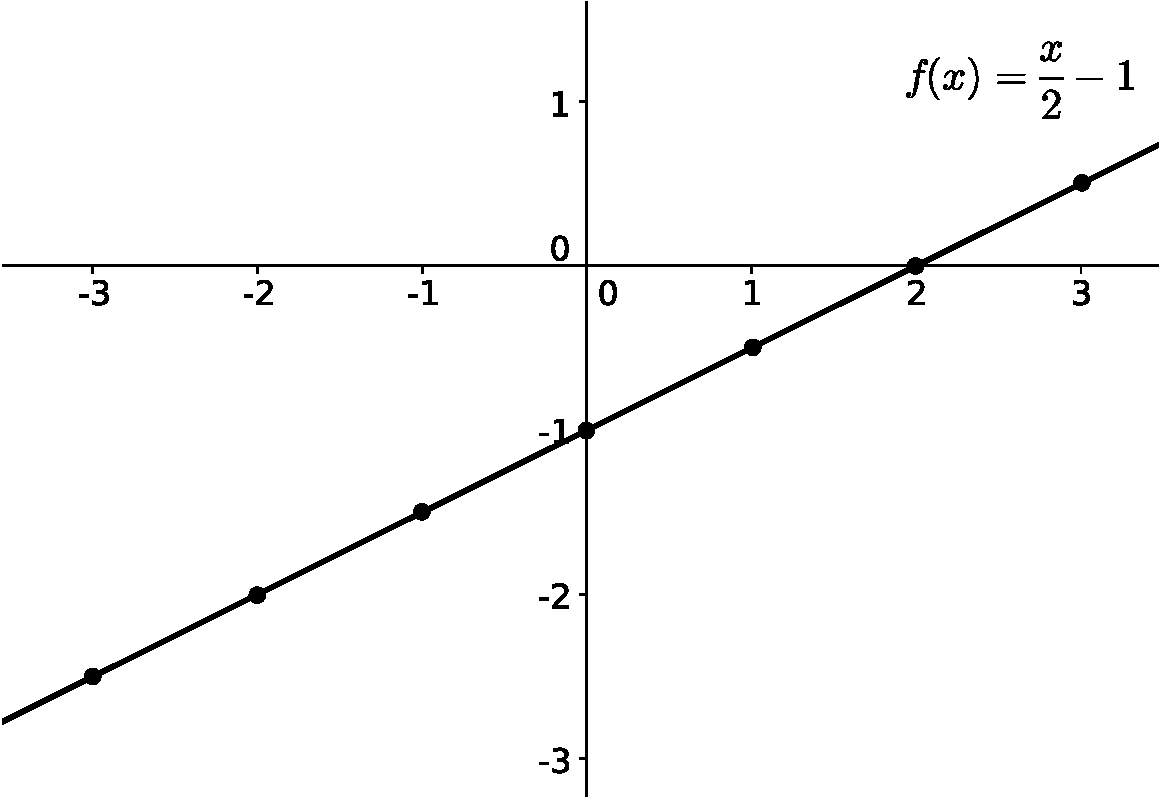
\includegraphics[width=0.5\textwidth, natwidth=220]{../kuvia/oppikirjamaraton/funktionkuvaaja/suoraesim-crop.pdf}}
\end{tabular}
\end{center}
\end{esimerkki}

\begin{esimerkki}
Funktion $f(x) = x^2$ kuvaaja sisältää kaikki pisteet $(x, y)$ joilla pätee $y = x^2$:
\begin{center}
\begin{tabular}{cc}
\begin{tabular}{|r|l|}
\hline
$x$ & $y = f(x)$ \\
\hline
$-2$ & $4$ \\
$-1$ & $1$ \\
$-0.5$ & $0.25$ \\
$0$ & $0$ \\
$0.5$ & $0.25$ \\
$1$ & $1$ \\
$2$ & $4$ \\
\hline
\end{tabular} &
%pikafiksi kuvakokoon, jotta kääntyy
\vcent{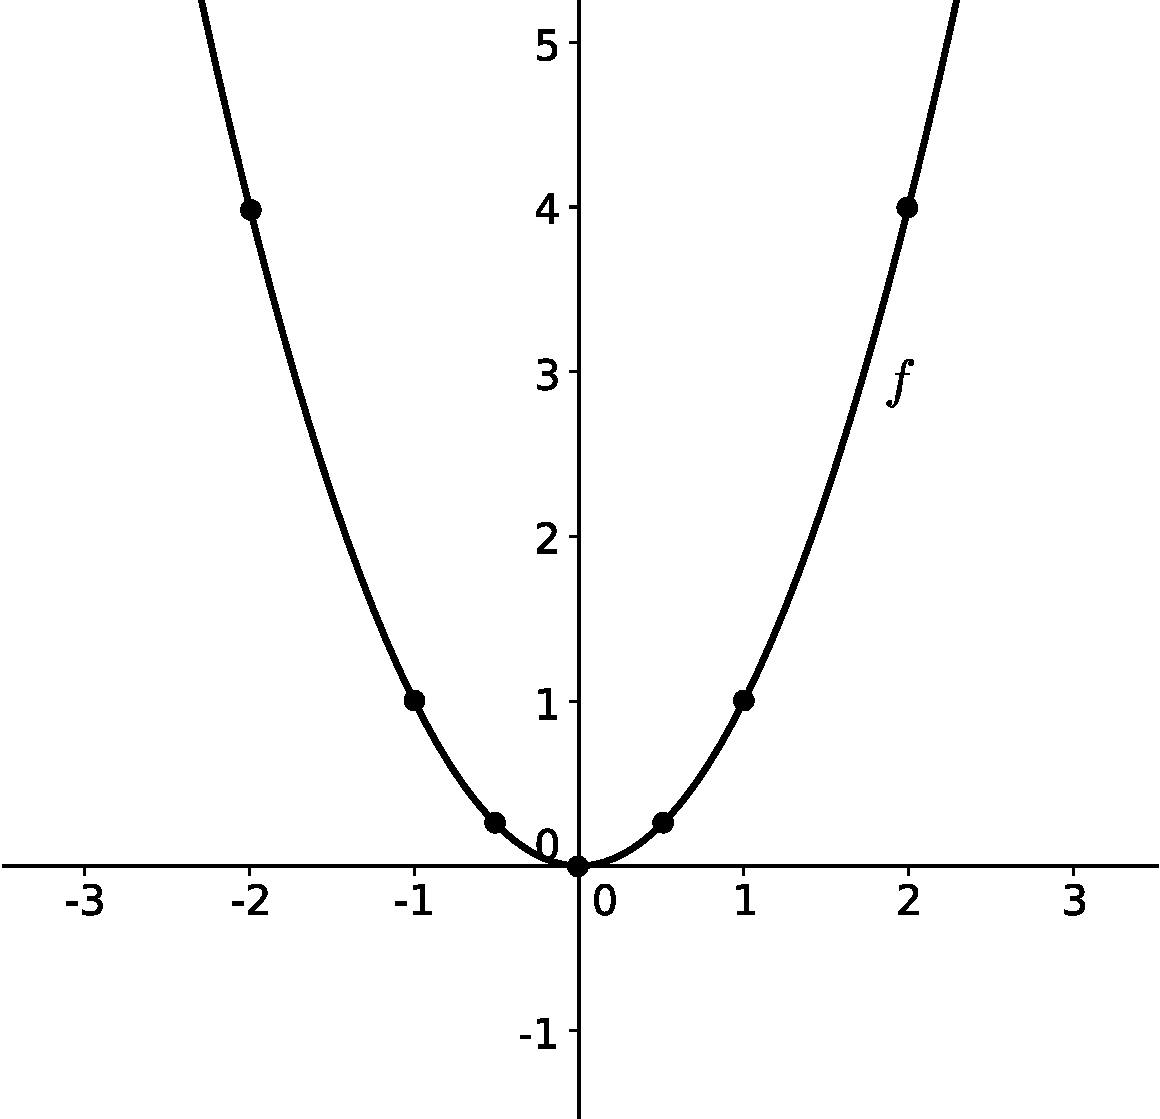
\includegraphics[width=0.5\textwidth, natwidth=220]{../kuvia/oppikirjamaraton/funktionkuvaaja/paraabeli-crop.pdf}}
\end{tabular}
\end{center}
\end{esimerkki}

\begin{esimerkki}
Funktion $f(x) = x^3-5x+2$ kuvaaja sisältää kaikki pisteet $(x, y)$ joilla pätee $y = x^2$:
\begin{center}
%pikafiksi kuvakokoon, jotta kääntyy
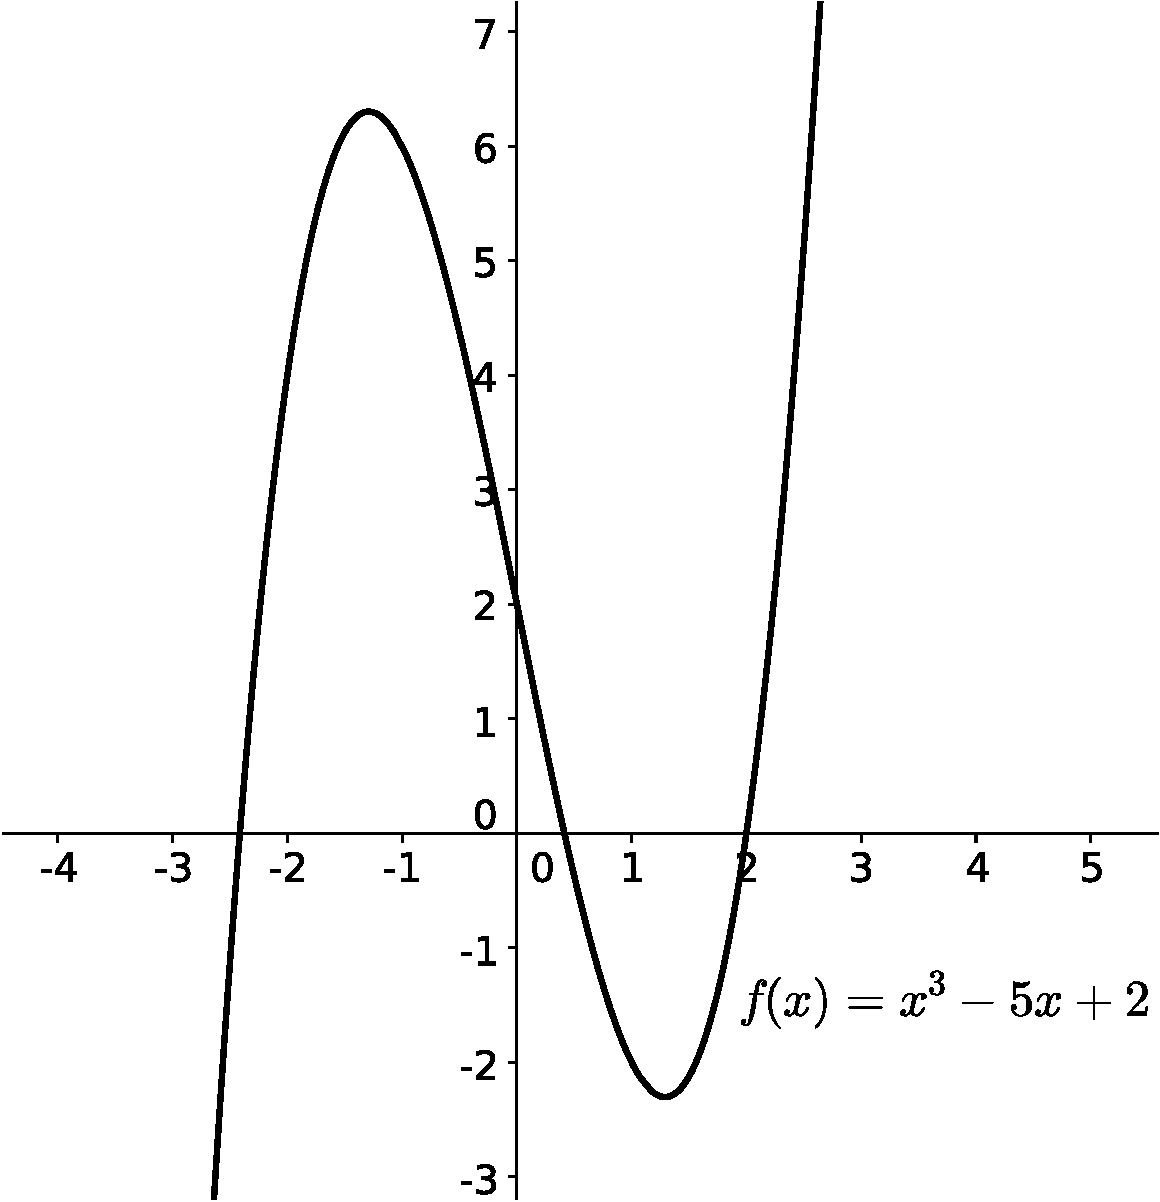
\includegraphics[width=0.5\textwidth, natwidth=220]{../kuvia/oppikirjamaraton/funktionkuvaaja/deg3polynomiesim-crop.pdf}
\end{center}
\end{esimerkki}

\section{Esimerkkejä funktioista}

\chapter{Potenssifunktio}

\chapter{Eksponenttifunktio}

Eksponenttifunktio on\ldots


\section{Eksponentiaalinen malli}

% Osan "Funktiot" kertaus.
\chapter{Kertaus}


\part{Kertaustehtäviä}
\chapter{''Näihin pystyt jo'' -yo-tehtäviä}

Ylioppilaskokeissa voi hyvinkin olla tehtäviä, joiden ratkaiseminen on mahdollista ja ensimmäisen matematiikan kurssin jälkeen.

\begin{description}

    \item[(K2012/1b)]  Ratkaise yhtälö
                        \[\frac{x}{6} - \frac{x-3}{2} - \frac{7}{9} = 0 \]
    \item[(K2012/2a)]  Laske lausekkeen $ \frac{15}{4} - \left( \frac{6}{3} \right)^2 $ arvo.
    \item[(S2011/1b)]  Ratkaise yhtälö
                        \[ \frac{4x - 1}{5} = \frac{x + 1}{2} + \frac{3 - x}{4} \]
    \item[(S2011/2a)]  Sievennä välivaiheet esittäen lauseke
                        \[ \frac{1}{\sqrt{2} + \frac{1}{2 + \sqrt{2}}} \]
    \item[(K2011/1a)]  Ratkaise yhtälö
                        \[ \frac{2}{x} = \frac{3}{x - 2} \]
    \item[(K2011/2a)]  Osakkeen arvo oli 35,50\,euroa. Se nousi ensin 12\,\%,
                        mutta laski seuraavana päivänä 10\%. Kuinka monta prosenttia
                        arvo nousi yhteensä näiden muutosten jälkeen?
    \item[(S2010/1a)]  Sievennä lauseke $ (a + b)^2 - (a - b)^2 $
    \item[(K2010/1b)]  Sievennä lauseke $ (\sqrt{a} + 1)^2 - a - 1 $
    \item[(S2009/1c)]  Osoita, että $ \sqrt{27 - 10 \sqrt{ 2} } = 5 - \sqrt{2} $
    \item[(S2009/2b)]  Ratkaise yhtälö $ \sqrt{x + 2 } = 3  $.
    \item[(K2009/1a)]  Sievennä $ \frac{a^2}{3} - \left( \frac{-a}{3} \right)^2 $
    \item[(S2008/1b)]  Sievennä lauseke
                        \[ \frac{1}{x} - \frac{1}{x^2} + \frac{1 + x}{x^2} \]
    \item[(S2009/2b)]  Ratkaise yhtälö
                        \[ \frac{x}{6} - \frac{x - 2}{3} = \frac{5}{12} \]
    \item[(K2008/4)]   Vuonna 2007 alennettiin parturimaksujen arvonlisäveroa 22
                        prosentista 8 prosenttiin. Jos alennus olisi siirtynyt
                        täysimääräisenä parturimaksuihin, kuinka monta prosenttia
                        ne olisivat alentuneet? Arvonlisävero ilmoitetaan prosentteina
                        verottomasta hinnasta ja se on osa tuotteen tai palvelun hintaa.
    \item[(S2007/1c)]  Ratkaise $L$ yhtälöstä
                        \[ t = \frac{1}{2\pi\sqrt{LC}} \]
    \item[(S2007/4)]   Tuotteen hintaa korotettiin $p$ prosenttia, jolloin menekki väheni.
                        Tämän johdosta hinta päätettiin alentaa takaisin alkuperäiseksi.
                        Kuinka monta prosenttia korotetusta hinnasta alennus oli?
    \item[(K2007/1c)]  Sievennä lauseke $ \sqrt[3]{a \sqrt{a}} \quad (a > 0) $.
    \item[(K2007/3a)]  Merivettä, jossa on 4,0 painoprosenttia suolaa, haihdutetaan
                        altaassa, kunnes sen massa on vähentynyt 28\,\%. Mikä on
                        suolapitoisuus haihduttamisen jälkeen? Anna vastaus prosentin
                        kymmenesosan tarkkuudella. 
    \item[(K2007/3b)]  Mikä on vuotuinen korkoprosentti, jos tilille talletettu rahamäärä
                        kasvaa korkoa korolle 1,5--kertaiseksi 10 vuodessa. Lähdeveroa
                        ei otetan huomioon. Anna vastaus prosentin sadasosan 
                        tarkkuudella.
    \item[(S2006/5)]   Hopean ja kuparin seoksesta tehty esine painaa 150\,g, ja sen
                        tiheys on 10,1\,kg/dm\(^3\). Kuinka monta painoprosenttia
                        esineessä on hopeaa ja kuinka monta kuparia, kun hopean tiheys on 
                        10,5\,kg/dm\(^3\) ja kuparin 9,0\,kg/dm\(^3\)?
    \item[(K2006/1a)]  Ratkaise $x$ yhtälöstä $4x + 2 =  3 - 2(x + 4)$.
    \item[(K2006/1c)]  Sievennä lauseke 
                        \[ \frac{1}{a - 1} \left( a - \frac{1}{a} \right) \]
    \item[(K2006/4)]   Kesämökin rakentaminen tuli 25\,\% arvioitua kalliimmaksi.
                        Rakennustarvikkeet olivat 19\,\% ja muut kustannukset 28\,\%
                        arvioitua kalliimpia. Mikä oli rakennustarvikkeiden arvioitu osuus ja 
                        mikä lopullinenosuus kokonaiskustannuksista?
    \item[(S2005/1a)]  Ratkaise reaalilukualueella yhtälö 
                        \[ 2(x - 1) + 3(x + 1 ) = -x \]
    \item[(S2005/1c)]  Ratkaise reaalilukualueella yhtälö $ x^{16} = 256 $.
    \item[(K2005/1a)]  Sievennä lauseke
                        \[ \frac{x}{1 - x} + \frac{x}{1 + x} \]
    \item[(K2005/2a)]  Ratkaise yhtälöryhmä
                        \[
                         \left\{
                         \begin{aligned}
                              x + y &= a \\
                              x - y &= 2a
                         \end{aligned}
                         \right.
                        \]
    \item[(K2005/3)]   Asuinrakennuksesta saadut vuokrat ovat 12\,\% pienemmät kuin
                        ylläpitokustannukset. Kuinka monta prosenttia vuokria olisi
                        korotettava, jotta ne tulisivat 10\,\% suuremmiksi kuin 
                        ylläpitokustannukset, jotka samanaikaisesti kohoavat 4\,\%?
    \item[(K2004/3)]   Perheen vuokramenot olivat 25\,\% tuloista. Vuokramenot nousivat
                        15\,\%. Montako prosenttia vähemmän rahaa riitti muuhun
                        käyttöön korotuksen jälkeen?
    \item[(S2003/5)]   Päärynämehusta ja omenamehusta tehdyn sekamehun sokeripitoisuus
                        on 11\,\%. Määritä mehujen sekoitussuhde, kun päärynämehun
                        sokeripitoisuus on 14\,\% ja omenamehun 7\,\%.
    \item[(S2003/12)]  Isä tallettaa poikansa tilille joka kuukauden alussa 200\,\euro \;
                        vuodenvaihteessa tapahtuneesta syntymästä alkaen. Tilille
                        maksetaan 1,5\,\% vuotuista korkoa, joka liitetään pääomaan aina 
                        vuoden lopussa.
                       
                        \begin{enumerate}[(a)]
                           \item Kuinka paljon rahaa tilillä on, kun poika täyttää
                                18 vuotta? 
                           \item Kuinka kauan isän olisi talletettava, jotta tilillä
                                olisi rahaa kaksiota varten, kun kaksion hinnaksi
                                oletetaan 135 000\,\euro ?
                        \end{enumerate}
                       
    \item[(K2003/1)]   Sievennä lausekkeet
        \begin{enumerate}[(a)]
            \item $ \sqrt{3\frac{3}{4}} \big/ \sqrt{1\frac{2}{3}} $
            \item $ \left( \frac{x}{y} + \frac{y}{x} -
                    2 \right) \big/ \left( \frac{x}{y} - \frac{y}{x} \right) $.
        \end{enumerate}
    \item[(S2002/2)]   Vuoden 1960 jälkeen on nopeimman junayhteyden matka-aika
                        Helsingin ja Lappeenrannan välillä lyhentynyt 37 prosenttia.
                        Laske, kuinka monta prosenttia keskinopeus on tällöin noussut.
                        Oletetaan, että radan pituus ei ole muuttunut.
    \item[(S2002/4a)]  Olkoon $ a \neq 0$ ja $b \neq 0 $. Sievennä lauseke
                        \[
                            \frac{a + \frac{b^2}{a} } {b + \frac{a^2}{b} }
                        \]
    \item[(K2002/3)]   Vuonna 2001 erään liikeyrityksen ulkomaille suuntautuvan
                        myynnin arvo kasvoi 10\,\% vuoteen 2000 verrattuna. Samaan
                        aikaan myynnin arvo kotimaassa väheni 5\,\%. Tällöin koko
                        myynnin arvo kasvoi 6\,\%. Laske, kuinka monta prosenttia
                        myynnistä meni vuonna 2000 ulkomaille.
    \item[(S2001/1)]   Ratkaise lineaarinen yhtälöryhmä
                       \[
                         \left\{
                          \begin{aligned}
                             3x - 2y &= 1 \\
                             4x + 5y &= 2                      
                         \end{aligned}
                         \right.
                       \]
    \item[(S2001/3)]   Juna lähtee Tampereelta klo 8.06 ja saapuu Helsinkiin klo 9.58.
                        Vastakkaiseen suuntaan kulkeva juna lähtee Helsingistä klo 8.58
                        ja saapuu Tampereelle klo 11.02. Matkan pituus on 187 kilometriä.
                        Oletetaan, että junat kulkevat tasaisella nopeudella, eikä
                        pysähdyksiin kuluvia aikoja oteta huomioon. Laske kummankin
                        junan keskinopeus. Millä etäisyydellä Helsingistä junat
                        kohtaavat, ja paljonko kello tällöin on? 
    \item[(K2001/4)]   Säiliö sisältää 2,3\,kg ilmaa, ja pumppu poistaa jokaisella
                        vedolla 5\,\% säiliössä olevasta ilmasta. Kunka monen vedon
                        jälkeen säiliössä on vähemmän kuin 0,2\,kg ilmaa?
    \item[(S2000/1)]   Sievennä seuraavat lausekkeet:
                        \begin{enumerate}[(a)]
                            \item $ \left( x^{n - 1} \right)^{n - 1} \cdot
                                \left( x^{n} \right)^{2 - n} $
                            \item $ \sqrt[3]{a} \; ( \sqrt[3]{a^2} - \sqrt[3]{a^5}) $
                        \end{enumerate}
    \item[(S2000/3)]   Matkaa kuljetaan tasaisella nopeudella. Kun matkasta on
                        jäljellä 40\,\%, nopeutta lisätään 20\,\%. Kuinka monta
                        prosenttia koko matkaan kuluva aika tällöin lyhenee?
    \item[(K2000/2)]   Lukion jazz--yhtyeen konsertin tuotto 192 euroa on jaettava
                        tasan yhtyeen jäsenille. Jos jäseniä olisi 2 enemmän, jokainen
                        saisi 8 euroa vähemmän. Montako jäsentä yhtyeessä on?

\end{description}

\chapter{Kurssiin liittyviä pääsykoetehtäviä}

\section{Arkkitehtivalinta}

\begin{description}
    \item[(2012/1)] Taloyhtiössä on $210$ asukasta. Taloyhtiö perii vesimaksua
        $15$ \euro/henkilö/kk. Kaupunki perii taloyhtiöltä vesimaksua
        kokonaiskulutuksen mukaan $3,17$ \euro $/ \mathrm{m}^3$.
        Taloyhtiön toteutunut kokonaisvedenkulutus on asukasta kohden
        155 litraa vuorokaudessa, mihin sisältyy hukkaan valuvia
        vuotoja yhtiötä kohden $1500 \mathrm{m}^3$ vuodessa. Oletamme,
        että vuodessa on $365$ vuorokautta.
                    
    \begin{enumerate}[(a)]
        \item Kuinka monta litraa vettä taloyhtiössä valuu hukkaan minuutissa?
        \item Vuodot tukitaan. Montako prosenttia vesimaksua voitaisiin laskea
            tai tulee korottaa, jotta vesimaksu tällöin kattaisi taloyhtiön
            vuotuiset vesikulut?
    \end{enumerate}
    
    Anna vastaukset kolmen numeron tarkkuudella.
\end{description}

% Vastaus: a) 2,85 l/min b) laskea 12,9 prosenttia

\begin{description}
    \item[(2010/3)] Arkkitehdit M. Uoto, F. Örm ja S. Hapé ovat suunnitelleet Aalto-yliopiston aulaan kullatusta teräskuutiosta muodostuvan taideteoksen. Kultaus on ohut.
    
    Toteutuksen aikana teoksen sijoituspaikka muuttuu, jolloin teräskuution tilavuutta kasvatetaan $19$\% alkuperäisestä. Loppulaskutuksessa materiaalikustannusten todetaan kasvaneen samaiset $19$\% alkuperäisestä budjetista.                   
    \begin{enumerate}[(a)]
        \item Paljonko kultaukseen käytetyn kullan määrä kasvoi toteutuksen aikana?
        \item Teräksen yksikköhinta ei toteutuksen aikana muuttunu. Miten kullan yksikköhinta siis muuttui?
    \end{enumerate}
    
    Anna vastaukset prosentteina $0,1$ prosenttiyksikön tarkkuuteen pyöristettynä.
\end{description}

\section{Diplomi-insinöörivalinta}
\begin{description}
	\item[(2012/3)] Asumistukea maksetaan 80 \% vuokran määrästä, siltä osin kuin
        vuokra ei ylitä 252 euroa. Vuokran määrää vähennettynä asumistuella
        kutsutaan omavastuuksi.
        
		\begin{enumerate}[(a)]
			\item Minka suuruinen vuokra on, kun omavastuu on puolet vuokrasta?
		\end{enumerate}
	
	\item[(2009/1)] Kokonaistuotanto jaetaan materian ja palveluiden tuotantoon.
        Verrataan tuotantoa tammikuussa 2008 tammikuuhun 2009. Tänä vuoden pituisen
        tarkastelujakson aikana materiatuotanto kasvoi 2,0 \% ja palvelutuotanto laski 7,0 \%.
	
	   Kuinka suuri oli materiatuotannon osuus kokonaistuotannosta tammikuussa 2009,
	   
    	\begin{enumerate}[(a)]
    		\item kun tammikuussa 2008 materia- ja palvelutuotanto olivat yhtäsuuret?
    		\item kun vertailuaikana kokonaistuotanto laski 2,0 \%?
    	\end{enumerate}
    	
	   Anna kummatkin vastaukset 0,1 \%-yksikön tarkkuuteen pyöristettynä.

	\item[(2008/2)] Yritys hankkii 5000 kg raaka-ainetta, josta on vettä 5,40 \%
        (painoprosenttia) ja väripigmenttiä 2,60 \%. Ennen käyttöä raaka-aine on
        laimennettava siten, että lisäyksen jälkeen sekoituksesta 6,60 \% on vettä.
	
    	\begin{enumerate}[(a)]
    		\item Miten paljon hankittuun raaka-aineeseen tulee lisätä vettä,
                jotta haluttu vesipitoisuus saavutetaan?
    		\item Miten paljon vettä ja väripigmenttiä tulee lisätä hankittuun
                raaka-aineeseen, jotta haluttu vesipitoisuus saavutetaan, ja lisäksi
                väripigmentin suhteellinen osuus massasta säilyy alkuperäisenä 2,60 \%:na?
    	\end{enumerate}
    	
    	Anna vastaukset sadan gramman tarkkuudella.

	\item[(2007/1)] Vaaleissa kaikkiaan 39 300 äänestäjästä 45 \% äänestää varmasti
        puoluetta A ja 47 \% puoluetta B. Loput ovat ns. liikkuvia äänestäjiä,
        jotka eivät ole vielä päättäneet kantaansa.
	
    	\begin{enumerate}[(a)]
    		\item Oletetaan, että kaikki äänioikeutetut äänestävät. Kuinka monta
                liikkuvien äänestäjien ääntä puolueen A täytyy tällöin kerätä
                saadakseen enemmistön, vähintään puolet annetuista äänistä?
    		\item Oletetaan, että täsmälleen kolmasosa liikkuvista äänestäjistä
                jättää äänestämättä. Kuinka monta prosenttia liikkuvien äänestäjien
                annetuista äänistä puolueen A täytyy tällöin kerätä saadakseen 
    		    enemmistön kaikista annetuista äänistä?
    	\end{enumerate}	 	
	
\end{description}

\section{Matematiikan ja tilastotieteen valinta}

\begin{description}
	\item[(2012/1a)] Ratkaise yhtälö $\frac{3}{2}x - \frac{2}{3} = \frac{2}{3}x - \frac{1}{4}$.
	\item[(2011/1)] Oletetaan, että polttoaineessa E05 on etanolia 5 \% ja
        bensiiniä 95 \% ja polttoaineessa E10 etanolia 10 \% ja bensiiniä 90 \%.
        Oletetaan myös, että etanolin energiasisältö on $\frac{2}{3}$ puhtaan bensiinin
		energiasisällöstä. Jos tietyllä autolla 100 km kulutus on 10 litraa
        polttoainetta E05, paljonko kulutus on polttoainetta E10? Anna vastaus
        sievennettynä murto- tai sekalukuna. Jos polttoaineen E10 hinta on 1,60 €/l
        ja polttoaineen E05 hinta on 1,65 €/l, kumpaa on edullisempaa käyttää?
	\item[(2008/1)] Matkailuauton nopeus on 80 km/h, mutta kolmasosalla matkasta
        Jyvaskylästä Heinolaan se laskee tietöiden takia 40 kilometriin tunnissa.
        Kuinka paljon tietyöt alentavat matkailuauton keskinopeutta valillä Jyväskylä-Heinola?
\end{description}

\section{Tekniikan ja liikenteen alan AMK-valinta}

\begin{description}
	\item[(K2012/3)] Erään tuotteen valmistuskustannuksista raaka-aineiden osuus on
        65 \% ja palkkojen osuus on 35 \%.
        
    	\begin{enumerate}[(a)]
    		\item Jos työntekijät saavat 5 \% palkankorotuksen, niin kuinka monta
                prosenttia tuotteen valmistuskustannukset kasvavat?
    		\item Jos toisaalta valmistuskustannukset halutaan pitää ennallaan
                palkankorotuksen jälkeen, niin montako prosenttia raaka-ainekustannusten
                pitää pienentyä?
    	\end{enumerate}	 

	\item[(K2012/4)] Esitä luku $\frac{1}{1+\frac{1}{1+\frac{1}{1+1}}}$ yhtenä murtolukuna (siis muodossa $\frac{m}{n}$).
	\item[(S2011/2)] Olkoon $a=132$ ja  $b=112$. Kuinka monta prosenttia 
		\begin{enumerate}[(a)]
			\item luku a on suurempi kuin luku b
			\item luku b on pienempi kuin luku a
			\item luku b on luvusta a? 
		\end{enumerate}
	\item[(K2011/1)] Laske lukujen $\frac{1}{3}$ ja $-\frac{7}{3}$
		\begin{enumerate}[(a)]
			\item summan vastaluku
			\item summan käänteisluku 
			\item käänteislukujen summa.
		\end{enumerate}
	\item[(K2011/2)] Yksi kilogramma etanolia tuottaa palaessaan energiaa 26,8 MJ
        ja vastaavasti yksi kilogramma puhdasta bensiiniä tuottaa palaessaan energiaa
        42,6 MJ. Kuinka monta prosenttia enemmän energiaa puhdas bensiini tuottaa
        palaessaan kuin 95 E10 -bensiini, joka sisältää 10 \% etanolia? Ilmoita
        vastaus yhden desimaalin tarkkuudella. 
\end{description}


\part{Liitteet}
\chapter{Lähtötasotesti}

(Tää tulee oikeasti ennen tätä chapteria ja osaa)

\begin{tehtava}
\begin{enumerate}
\item Laske $2^2+2 \cdot 2+2$
\item sasdas
\item 
\end{enumerate}

\begin{vastaus}
\begin{enumerate}
\item 
\item
\item

\end{enumerate}
\end{vastaus}
\end{tehtava}

\chapter{Suureista ja yksiköistä}

\begin{tehtava}
Muuta minuuteiksi
\begin{enumerate}
\item $1$ h $17$ min
\item $2$ h $45$ min
\item $1,5$ h
\item $1,75$ h
\end{enumerate}
\begin{vastaus}
\begin{enumerate}
\item $77$ min
\item $165$ min
\item $90$ min
\item $105$ min
\end{enumerate}
\end{vastaus}
\begin{tehtava}

\begin{tehtava}
Muuta tunneiksi ja minuuteiksi
\begin{enumerate}
\item $125$ min
\item $667$ min
\item $120$ min
\item $194$ min
\end{enumerate}
\begin{vastaus}
\begin{enumerate}
\item $2$ h $5$ min
\item $11$ h $7$ min
\item $2$ h
\item $3$ h $14$ min
\end{enumerate}
\end{vastaus}
\begin{tehtava}
% Tähän tulee liitteitä
% Esimerkiksi loogiset symbolit, reaalilukujen aksioomat, kompleksilukuintro, ...
\part{Liiteet}
% Vaihda tähän kirjaimin kulkeva "numerointi"
\chapter{Logiikka ja joukko-oppi}
\chapter{Reaalilukujen aksioomat}
Reaaliluvut ovat kunta, eräs algebrallinen rakenne. Myös esimerkiksi rationaaliluvut ja seuraavassa liitteessä esiteltävät kompleksiluvut muodostavat kunnan. Sen sijaan luonnolliset luvut ja kokonaisluvut eivät ole kuntia.

Reaalilukujen aksiomaattinen määritelmä muodostuu kolmesta osasta:

% Pitäisikö 'kunta-aksioomat' erottaa 'kunta-aksioomista reaalilukujen tapauksessa'

\begin{align*}
&\textbf{Kunta-aksioomat} \\
&\textbf{K1.} \, \forall x, y \in \mathbb{R}: & &x+(y+z) = (x+y)+z & &| \, \text{summan liitäntälaki} \\
&\textbf{K2.} \, \exists 0 \in \mathbb{R}: & &x+0 = x & &| \, \text{summan neutraalialkio} \\
&\textbf{K3.} \, \forall x \in \mathbb{R} & &\exists (-x) \in \mathbb{R}: \quad x+(-x)=0 & &| \, \text{vasta-alkio} \\
&\textbf{K4.} \, \forall x, y \in \mathbb{R}: & &x+y = y+x & &| \, \text{summan vaihdantalaki} \\
&\textbf{K5.} \, \forall x, y, z \in \mathbb{R}: & &x \cdot (y+z) = x \cdot y + x \cdot z & &| \, \text{osittelulaki} \\
&\textbf{K6.} \, \forall x, y, z \in \mathbb{R}: & &x \cdot (y \cdot z) = (x \cdot y) \cdot z & &| \, \text{tulon liitäntälaki} \\
&\textbf{K7.} \, \exists 1 \in \mathbb{R}: & &1 \cdot x = x & &| \, \text{tulon neutraalialkio} \\
&\textbf{K8.} \, \forall x \in \mathbb{R} \setminus \{0\} & &\exists x^{-1} \in \mathbb{R} \setminus \{0\}: \quad x \cdot x^{-1}=1 & &| \, \text{tulon käänteisalkio} \\
&\textbf{K9.} \, \forall x, y \in \mathbb{R}: & &x \cdot y = y \cdot x & &| \, \text{tulon vaihdantalaki} \\
&\textbf{Järjestysaksioomat} \\
&\textbf{J1.} \, \forall x, y \in \mathbb{R}: & &\text{täsmälleen yksi seuraavista:} & \\
& & &(x > y), \, (x = y), \, (x < y) & \\
&\textbf{J2.} \, \forall x, y, z \in \mathbb{R}: & &(x < y) \land (y < z) \Rightarrow (x < z) & \\
&\textbf{J3.} \, \forall x, y, z \in \mathbb{R}: & &(x < y) \Leftrightarrow (x + z < y + z) & \\
&\textbf{J4.} \, \forall x, y \in ]0,\infty[: & &x \cdot y \in ]0,\infty[ & \\
&\textbf{Täydellisyysaksiooma}
\end{align*}
% Kuinka saadaan seuraava rivi alignin sisään ilman että kaikki hajoaa?:
\textbf{T1.} \, Jokaisella ylhäältä rajoitetulla epätyhjällä reaalilukujen osajoukolla on pienin yläraja.

\Closesolutionfile{ans} % Answers-ratkaisut
\chapter{Ratkaisut}
\begin{Vastaus}{1}
Esimerkkivastaus.
\end{Vastaus}
\begin{Vastaus}{2}
$3$
\end{Vastaus}
\begin{Vastaus}{3}
$x=-1$
\end{Vastaus}
\begin{Vastaus}{4}
\begin{enumerate}
\item
\item
\item

\end{enumerate}
\end{Vastaus}
\begin{Vastaus}{6}
        a) $\frac{18}{5}$
        b) $\frac{5}{8}$
        c) $3$
        d) $-\frac{41}{6}$
    
\end{Vastaus}
\begin{Vastaus}{7}
        a) $\frac{2}{5}$
        b) $\frac{5}{6}$
        c) $\frac{1}{2}$
        d) $\frac{1}{8}$
    
\end{Vastaus}
\begin{Vastaus}{8}
        a) $\frac{47}{28}$
        b) $\frac{1}{2}$
        c) $-\frac{1}{3}$
        d) $\frac{54}{5}$
    
\end{Vastaus}
\begin{Vastaus}{9}
        Muut saavat piirakasta kuudesosan.
    
\end{Vastaus}
\begin{Vastaus}{10}
        37,50 euroa
    
\end{Vastaus}
\begin{Vastaus}{11}
a) $a^3$ \qquad b) $a^3b^4$ \qquad c) $a^4b^3$
\end{Vastaus}
\begin{Vastaus}{12}
a) $a^5$ \qquad b) $a^5$ \qquad c) $a^3$ \qquad d) $a^4$ \qquad e) $a^6$
\end{Vastaus}
\begin{Vastaus}{13}
a) $1$ \quad ($a\neq0$, koska $0^0$ ei ole määritelty) \qquad b) $1$ \qquad c) $a$ \qquad d) $a^2$ \qquad
e) $a$
\end{Vastaus}
\begin{Vastaus}{14}
a) $ a^4$ \qquad b) $a^4$ \qquad c) $a^5b$ \qquad d) $a^2b^2$
\end{Vastaus}
\begin{Vastaus}{15}
a) $ -8$ \qquad b) $1$
\end{Vastaus}
\begin{Vastaus}{16}
a) $a^2$ \qquad b) $-a^2b$ \qquad c) $a^4$
\end{Vastaus}
\begin{Vastaus}{17}
a) $a^2$ \qquad b) $-a^2b$ \qquad c) $a^4$
\end{Vastaus}
\begin{Vastaus}{18}
a) $a^5$ \qquad b) $a^2b$ \qquad c) $-a^4$
\end{Vastaus}
\begin{Vastaus}{19}
a) $64$ \qquad b) $64$ \qquad c) $64$ \qquad d) $64$
\end{Vastaus}
\begin{Vastaus}{20}
a) $1$ \qquad b) $3$ \qquad c) $32$ \qquad d) $4$ \qquad e) $1$
\end{Vastaus}
\begin{Vastaus}{21}
a) $a^3$ \qquad b) $a^{12}$ \qquad c) $a^8$ \qquad d) $a^3$ \qquad e) $1$
\end{Vastaus}
\begin{Vastaus}{22}
a) $a^{10}$ \qquad b) $a^6$ \qquad c) $a^{20}$ \qquad d) $a^5$
\end{Vastaus}
\begin{Vastaus}{23}
a) $a^3$ \qquad b) $4a^2$ \qquad c) $-8a^3b^3c^3$ \qquad d) $91a^4$
\end{Vastaus}
\begin{Vastaus}{24}
a) $a^8b^2$ \qquad b) $a^2b^6$ \qquad c) $a^{15}b^{12}$ \qquad d) $a^2b^3$
\end{Vastaus}
\begin{Vastaus}{25}
a) $a^2b^3$ \qquad b) $1$ \qquad c) $a^{17}$ \qquad d) $a^8b^{10}$
\end{Vastaus}
\begin{Vastaus}{26}
a) $16$ \qquad b) $64$ \qquad c) $16a^8$ \qquad d) $27b^4$
\end{Vastaus}
\begin{Vastaus}{27}
a) $a^6b^4$ \qquad b) $a^9b^{12}$ \qquad c) $a^{20}b^{10}$ \qquad d) $8a^3b^7$
\end{Vastaus}
\begin{Vastaus}{28}
a) $2$ \qquad b) $4$ \qquad c) $4$ \qquad d) $8$ \qquad e) $\frac{1}{2}$ \qquad f) $\frac{1}{4}$
\end{Vastaus}
\begin{Vastaus}{29}
a) $a$ \qquad b) $a^2$ \qquad c) $a^2$ \qquad d) $a^3$ \qquad e) $a^{-1} = \frac{1}{a}$ \qquad f) $a^{-2} = \frac{1}{a^2}$
\end{Vastaus}
\begin{Vastaus}{30}
a) $ab$ \qquad b) $b$ \qquad c) $1$ \qquad d) $1$ \qquad e) $-\frac{a}{b}$
\end{Vastaus}
\begin{Vastaus}{31}
a) $\frac{1}{a^3}$ \qquad b) $\frac{1}{a^2}$ \qquad c) $a^3$ \qquad d) $\frac{}{a^4b^3}$ \qquad e) $a^8$
\end{Vastaus}
\begin{Vastaus}{32}
a) $\frac{1}{4}$ \qquad b) $\frac{1}{27}$ \qquad c) $\frac{a^4}{b^4}$ \qquad d) $\frac{a^4}{b^6}$ \qquad e) $\frac{a^2}{b^4}$
\end{Vastaus}
\begin{Vastaus}{33}
a) $\frac{1}{4}$ \qquad b) $-\frac{b^3}{a^3}$ \qquad c) $a^8b^8$ \qquad d) $\frac{a^8}{b^8}$
\end{Vastaus}
\begin{Vastaus}{34}
a) $2a^7$ \qquad b) $b^9$ \qquad c) $-\frac{1}{3}a = -\frac{a}{3}$ \qquad d) $\frac{10\ 000}{b^6}$
\end{Vastaus}
\begin{Vastaus}{35}
\begin{enumerate}
\item $2x^2$
\item $3+4y$
\item $ -\frac{x}{6}$
\item $ \frac{2}{3} x - \frac{17}{6}$
\end{enumerate}
\end{Vastaus}


\chapter{Tekijät}
